%%%%%%%%%%%%%%%%%%%%%%%%%%%%%%%%%%%%%%%%%%%%%%%%%%%%%%%%%%%%%%%%%%%%%%%%%%%%%%%
% Settings - DO NOT CHANGE
%%%%%%%%%%%%%%%%%%%%%%%%%%%%%%%%%%%%%%%%%%%%%%%%%%%%%%%%%%%%%%%%%%%%%%%%%%%%%%%
\documentclass[10pt,a4paper]{article}
\usepackage{amsmath}
\usepackage{amsfonts}
\usepackage{amssymb}
\usepackage{graphicx}
\usepackage{float}
%\usepackage{fontspec}
\graphicspath{{assets/}}
\usepackage[margin=0.75in]{geometry}
\usepackage{fontspec}
\usepackage{blindtext}
\setmainfont{ScalaSansPro-Regular.otf}[
BoldFont = ScalaSansPro-Bold.otf,
ItalicFont = ScalaSansPro-Italic.otf,
BoldItalicFont  = ScalaSansPro-BoldItalic.otf]
\usepackage{caption}
\captionsetup{justification=raggedright,singlelinecheck=false}
\usepackage{subfig}
\usepackage{listings}
\usepackage{color}

\definecolor{dkgreen}{rgb}{0,0.6,0}
\definecolor{gray}{rgb}{0.5,0.5,0.5}
\definecolor{mauve}{rgb}{0.58,0,0.82}
\definecolor{lblue}{RGB}{127, 197, 220}
\definecolor{lred}{RGB}{249, 3, 36}
\definecolor{lgray}{rgb}{0.9,0.9,0.9}

\lstset{frame=tb,
  language=Python, % Change this if you want to include code other than Python globally
  aboveskip=3mm,
  belowskip=3mm,
  showstringspaces=false,
  columns=flexible,
  basicstyle={\small\ttfamily},
  numbers=none,
  numberstyle=\tiny\color{red},
  keywordstyle=\color{lblue},
  commentstyle=\color{gray},
  stringstyle=\color{lred},
  breaklines=true,
  breakatwhitespace=true,
  tabsize=3}
\usepackage[table]{xcolor}
\usepackage{array}

%%%%%%%%%%%%%%%%%%%%%%%%%%%%%%%%%%%%%%%%%%%%%%%%%%%%%%%%%%%%%%%%%%%%%%%%%%%%%%%

\begin{document}

\vspace*{-4\baselineskip}
\begin{figure}[h!]
	\hspace{65pt}
	
\includegraphics[width=0.3\linewidth]{logo}
	\vspace*{-11\baselineskip}
\end{figure}

\begin{center}
    \vspace*{2.25\baselineskip}
    \hspace*{190pt}
    \large\textbf{Paper }\text{Computer Science 101} \\ % Put Paper Name Here
    \hspace*{225pt}
    \large\textbf{Topic }\text{CUDA/C++ Coding Principles} \\ % Put Assignment Topic/Name Here
    \hspace*{180pt}
    \large\textbf{Lecturer(s) }\text{Lecturer Name} \\ % Lecturer Name
   	\hspace*{165pt}
    \large\textbf{Due }\text{3:00pm 29/1/1992} \\ % Due time/date
\end{center}
\vspace*{2\baselineskip}
\par\noindent\rule{\textwidth}{0.01pt}

% DO NOT MODIFY
\begin{center}
	\vspace*{1\baselineskip}
	\textbf{Name } \rule{132pt}{0.1pt} \\
	\vspace*{1\baselineskip}
	\textbf{Student ID } \rule{112pt}{0.1pt} \\
	\vspace*{1\baselineskip}

\par\noindent\rule{\textwidth}{0.01pt}


%%%%%%%%%%%%%%%%%%%%%%%%%%%%%%%%%%%%%%%%%%%%%%%%%%%%%%%%%%%%%%%%%%%%%%%%%%%%%%%
% You can modify the instructions here
%%%%%%%%%%%%%%%%%%%%%%%%%%%%%%%%%%%%%%%%%%%%%%%%%%%%%%%%%%%%%%%%%%%%%%%%%%%%%%%
\vspace*{1.5\baselineskip}
\centering\large\textbf{Instructions}

\vspace*{1\baselineskip}
\hspace*{225pt}
\begin{enumerate}
	\item Read all the questions carefully.
	\item Solve all the questions.
	\item Submit assignment.
    \item 
    \item
\end{enumerate}
\par\noindent\rule{\textwidth}{0.01pt}

%%%%%%%%%%%%%%%%%%%%%%%%%%%%%%%%%%%%%%%%%%%%%%%%%%%%%%%%%%%%%%%%%%%%%%%%%%%%%%%
% You can modify the grading here
%%%%%%%%%%%%%%%%%%%%%%%%%%%%%%%%%%%%%%%%%%%%%%%%%%%%%%%%%%%%%%%%%%%%%%%%%%%%%%%
\vspace*{1.5\baselineskip}
%\centering\large\textbf{Grading Section}

%\vspace*{1\baselineskip}
%{0, 140, 186}
\setlength{\tabcolsep}{18pt}
\newcolumntype{M}[1]{>{\centering\arraybackslash}m{#1}}
\newcolumntype{N}{@{}m{0pt}@{}}
%\rowcolors{2}{lblue}{lgray}

\begin{tabular}{|M{2cm}|M{2cm}|M{2cm}|N}
 	\hline
 	%\cellcolor[HTML]{7FC5DC}\textbf{Question} & 
    %\cellcolor[HTML]{7FC5DC}\textbf{Grade} & 
    %\cellcolor[HTML]{7FC5DC}\textbf{Score} &\\[10pt] \hline
    \cellcolor[HTML]{7FC5DC}\textbf{Question} & \cellcolor[HTML]{7FC5DC}\textbf{Grade} & \cellcolor[HTML]{7FC5DC}\textbf{Score} &\\[10pt] \hline
    Q.1 & 10 &  &\\ [7pt] \hline
 	Q.2 & 10 &  &\\ [7pt] \hline
 	Q.3 & 10 &  &\\ [7pt] \hline
 	Q.4 & 10 &  &\\ [7pt] \hline
 	Q.5 & 10 &  &\\ [7pt] \hline
 	Q.6 & 10 &  &\\ [7pt] \hline
 	Q.7 & 10 &  &\\ [7pt] \hline
 	Q.8 & 10 &  &\\ [7pt] \hline
    Q.9 & 10 &  &\\ [7pt] \hline
 	Q.10 & 10 &  &\\ [7pt] \hline
    \cellcolor[HTML]{7FC5DC}\textbf{Total} & \cellcolor[HTML]{7FC5DC}\textbf{100} & \cellcolor[HTML]{7FC5DC} &\\[10pt] \hline
    
\end{tabular}

\end{center}
%\vspace*{1\baselineskip}
%\par\noindent\rule{\textwidth}{0.01pt}
%%%%%%%%%%%%%%%%%%%%%%%%%%%%%%%%%%%%%%%%%%%%%%%%%%%%%%%%%%%%%%%%%%%%%%%%%%%%%%%
% First Page of Assignment
%%%%%%%%%%%%%%%%%%%%%%%%%%%%%%%%%%%%%%%%%%%%%%%%%%%%%%%%%%%%%%%%%%%%%%%%%%%%%%%
% Create sections and pages like such:
\newpage
\section*{Question 1}

% \\ shifts to a new line
In essence, technical neural networks are radically generalized forms of organic/biological neural networks. They are mathematical representations of the functions of nerve cells. \\


% You can force the text to align left with  \flushleft
% You can write an equation in-line using $x$ notation
\flushleft{A very simple neuron receives a vector input, with components $x_i$} \\

% or to the right \flushright
\flushright{A very simple neuron receives a vector input, with components $x_i$} \\

% You can also create centered text
\centering{A very simple neuron receives a vector input, with components $x_i$} \\

% or with \begin{center} and \end{center} if multiple items
\begin{center}
This is centered \\
This is also centered
\end{center}



% You can create bold text by using \textbf{My Text}
\flushleft\textbf{BOLD TEXT} \\

% You can create italic text by using \textit{MyText}
\flushleft\textit{ITALIC TEXT} \\

% You can write equations on separate lines using $$x$$
$$
\vec{x}
$$

The inputs are multiplied by the weightings $w_i$, and accumulated into a \emph{weighted sum}.
% or using \[x\]
\[\sum_i{w_ix_i}\]

Then, $f$ is non-linearly mapped to define the scalar output $y$ as:

% You can also include equation numbering if you enclose the equation with \begin{equation} and \end{equation}
\begin{equation}
y = f(\sum_i{w_ix_i})
\end{equation}

% This is how you can create bullet points and numbering
\section*{Question 2}
\begin{enumerate}
	\item{Item 1}
    \begin{itemize}
    	\item{Sub-Item 1}
        \begin{enumerate}
        	\item{Sub-sub-item 1}
        \end{enumerate}
    \end{itemize}
    \item{Item 3}
\end{enumerate}

%%%%%%%%%%%%%%%%%%%%%%%%%%%%%%%%%%%%%%%%%%%%%%%%%%%%%%%%%%%%%%%%%%%%%%%%%%%%%%%
% You can insert figures with 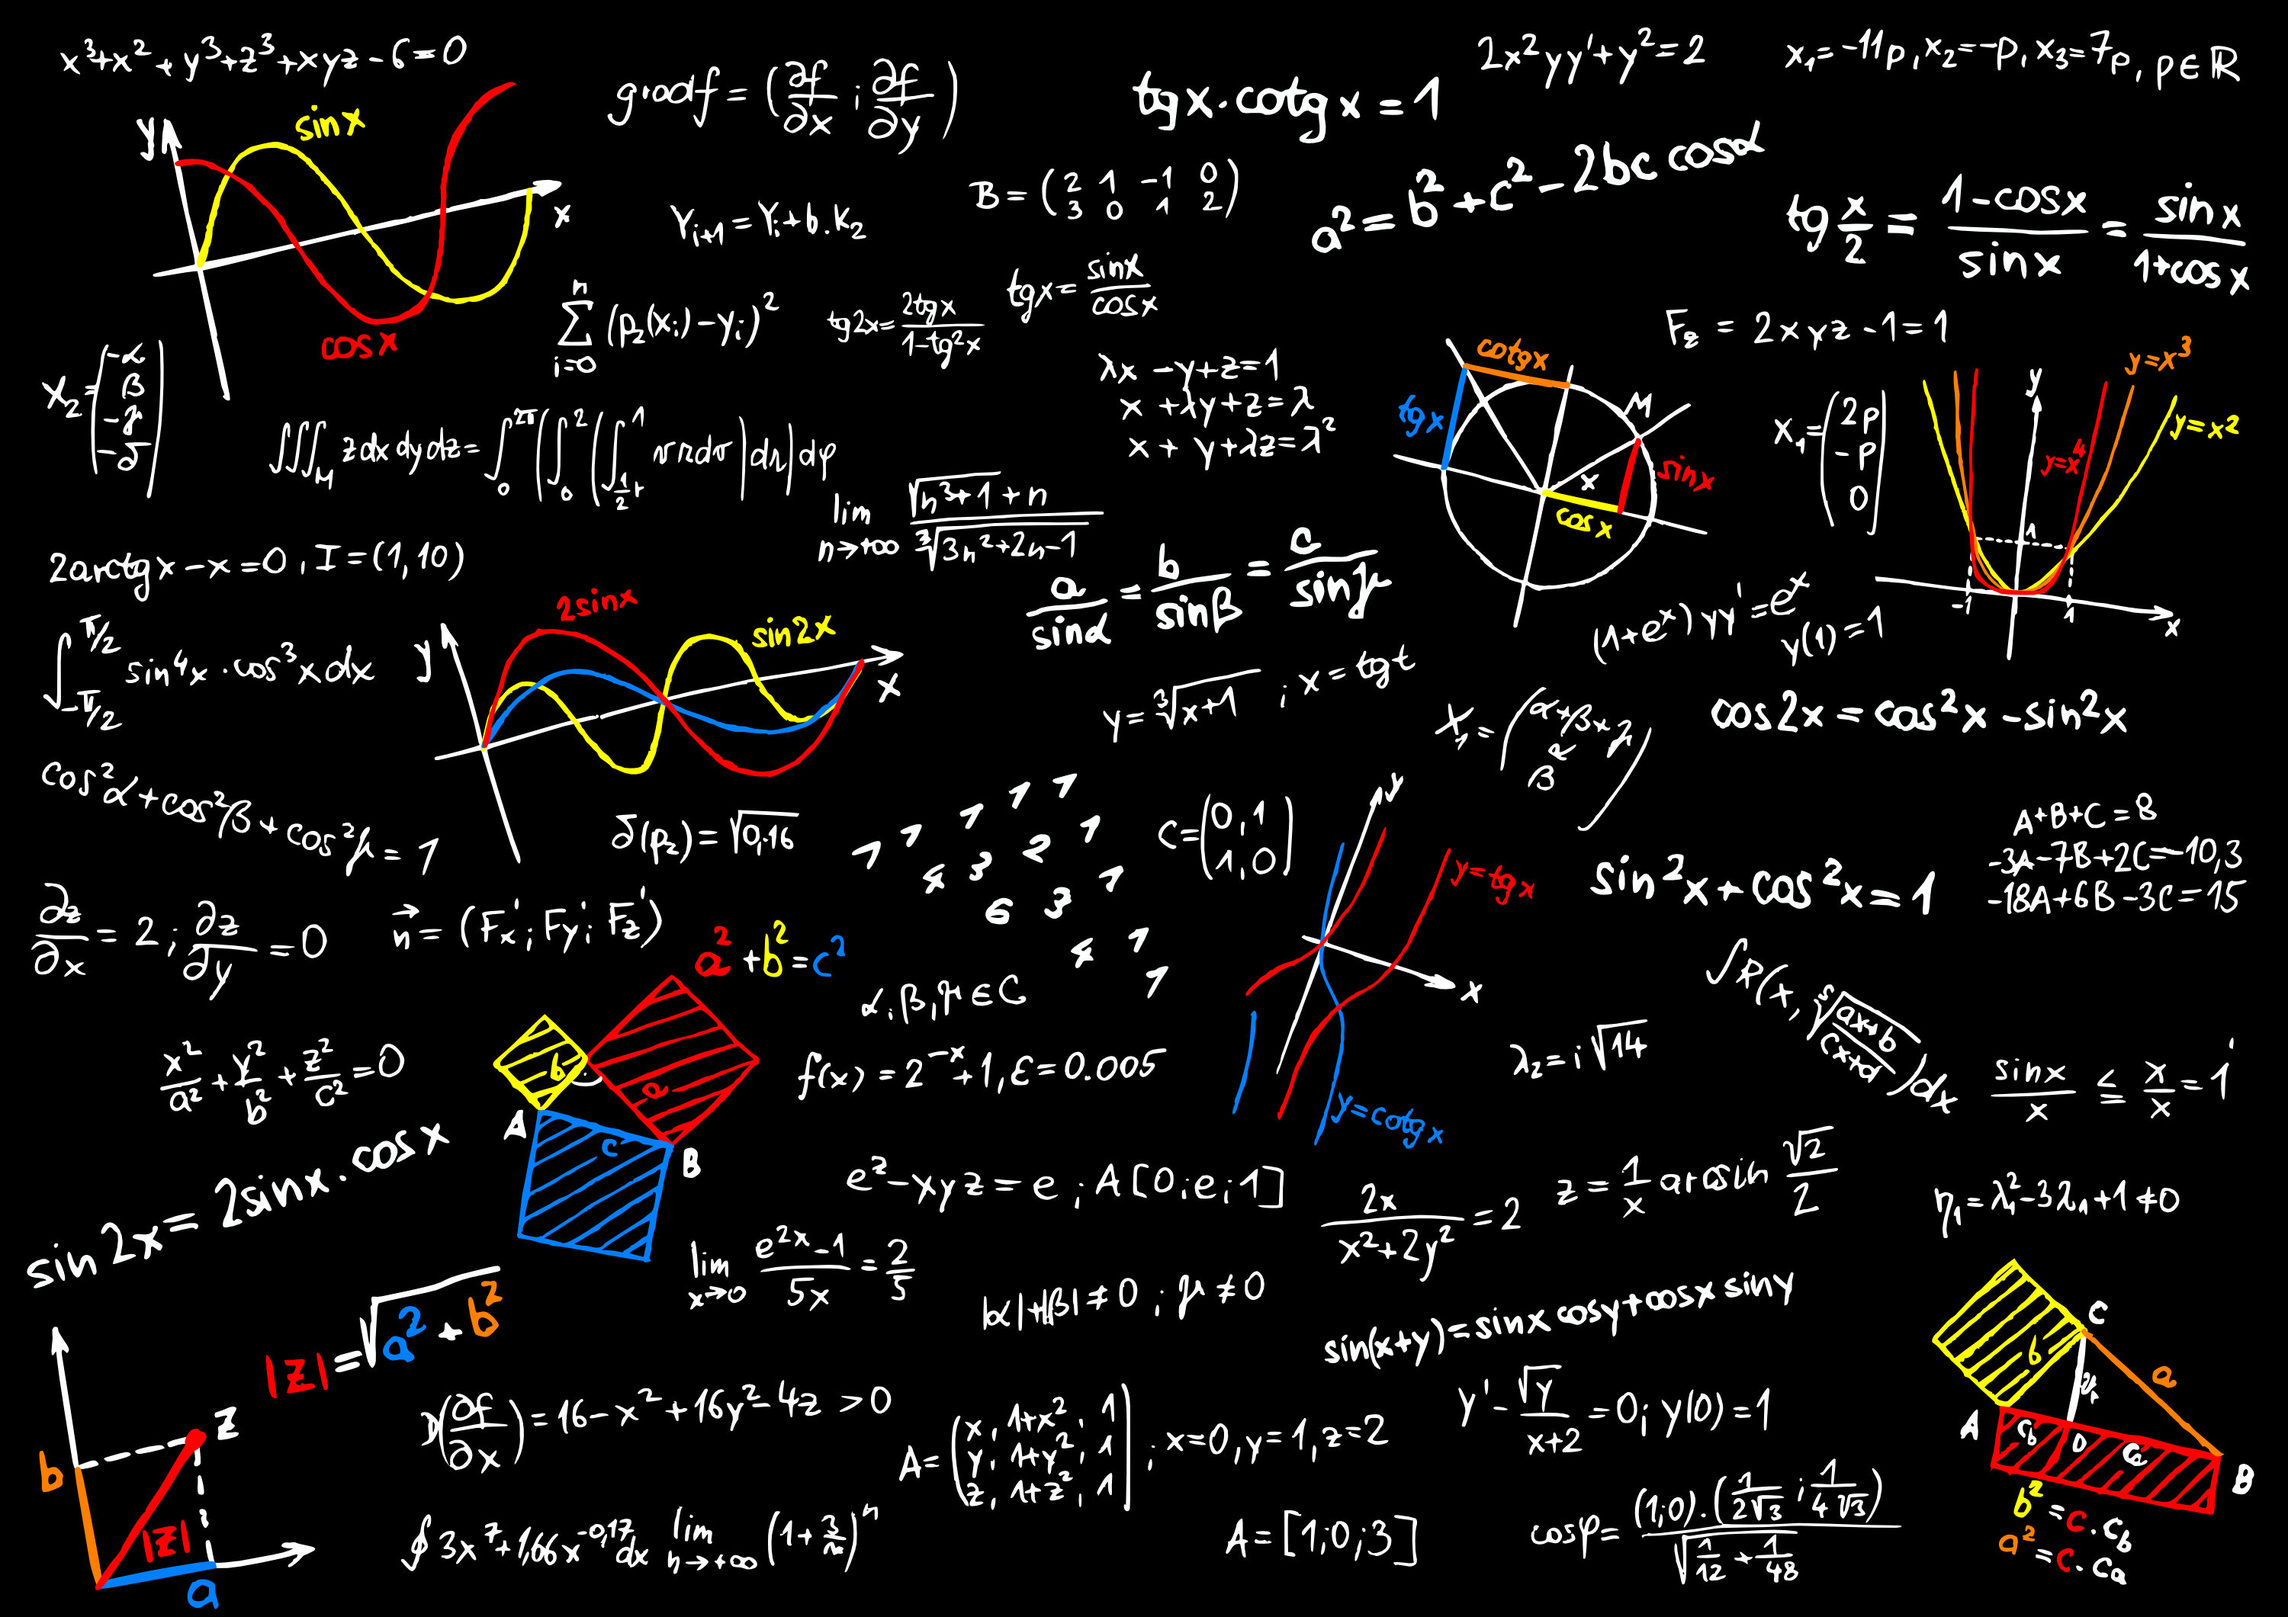
\includegraphics[width=??\linewidth]{math}
%%%%%%%%%%%%%%%%%%%%%%%%%%%%%%%%%%%%%%%%%%%%%%%%%%%%%%%%%%%%%%%%%%%%%%%%%%%%%%%
% When you add a caption, they are automatically named and numbered Figure 1, Figure 2, etc..
\newpage
\section*{Figures}
\textbf{1. You can insert figures of different sizes:}
\begin{figure}[h!]
	% To include a figure with filename math.jpg, there is no need to write the extension .jpg
	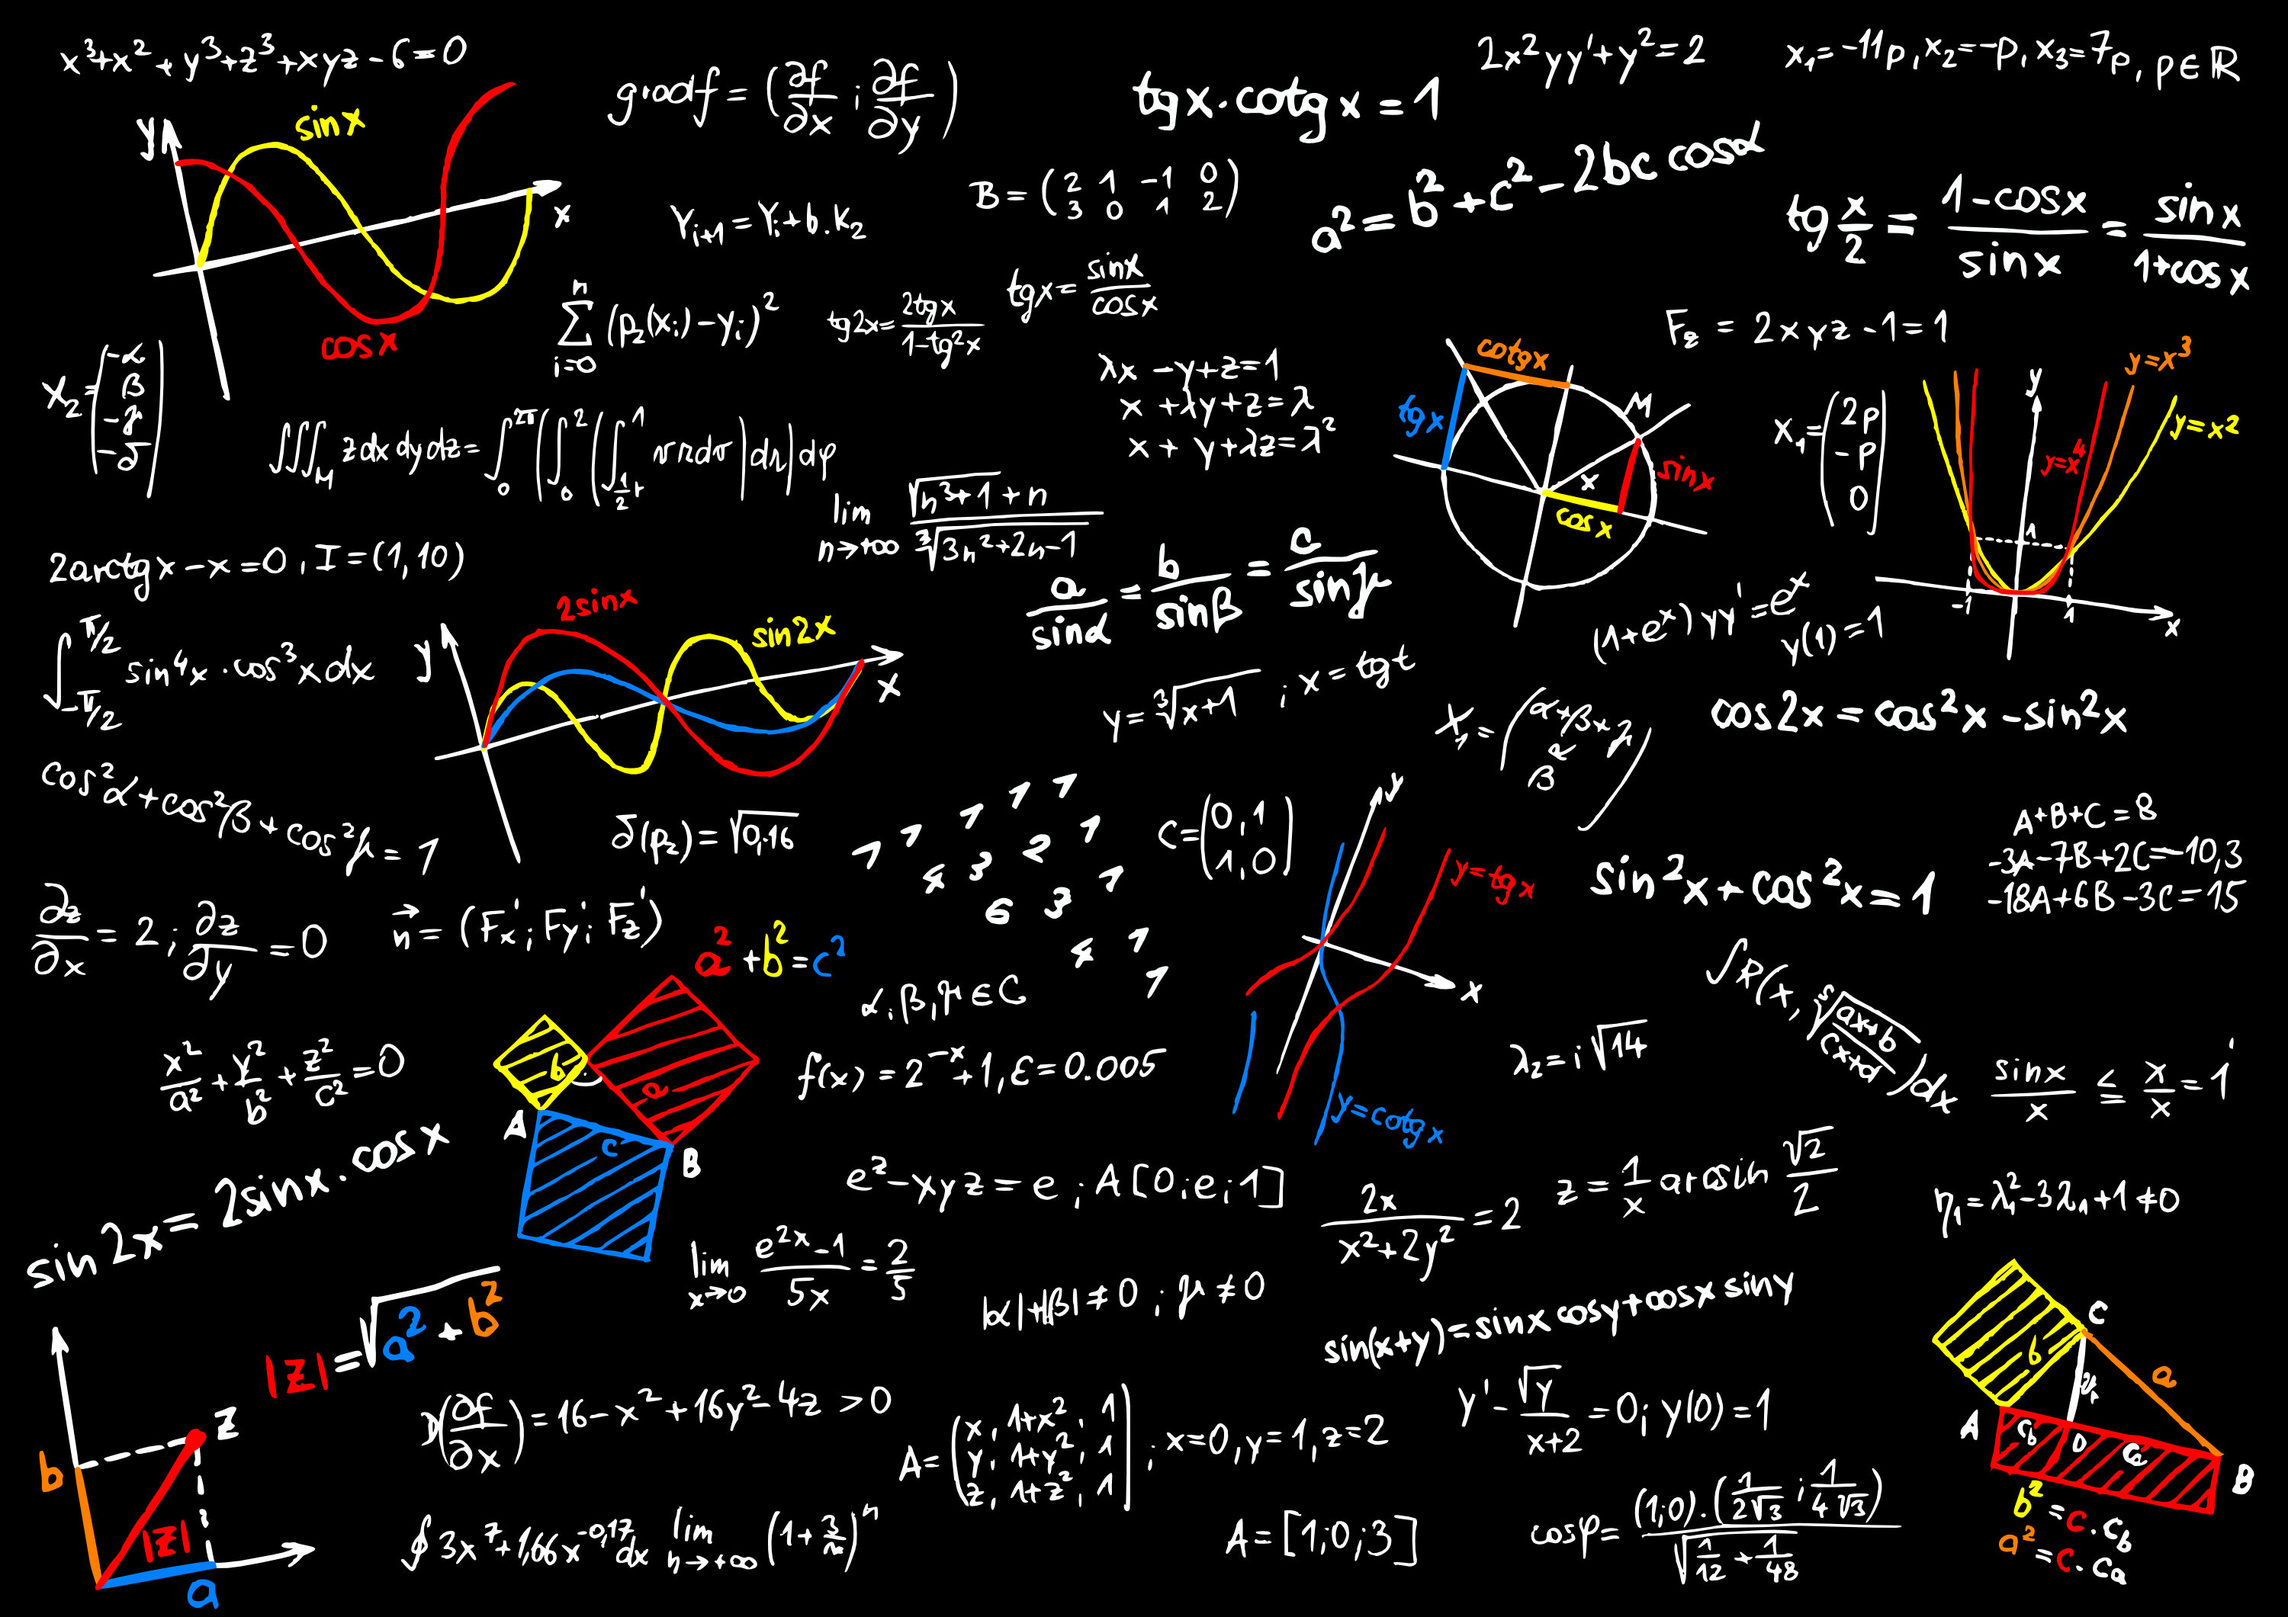
\includegraphics[width=0.5\linewidth]{math}
	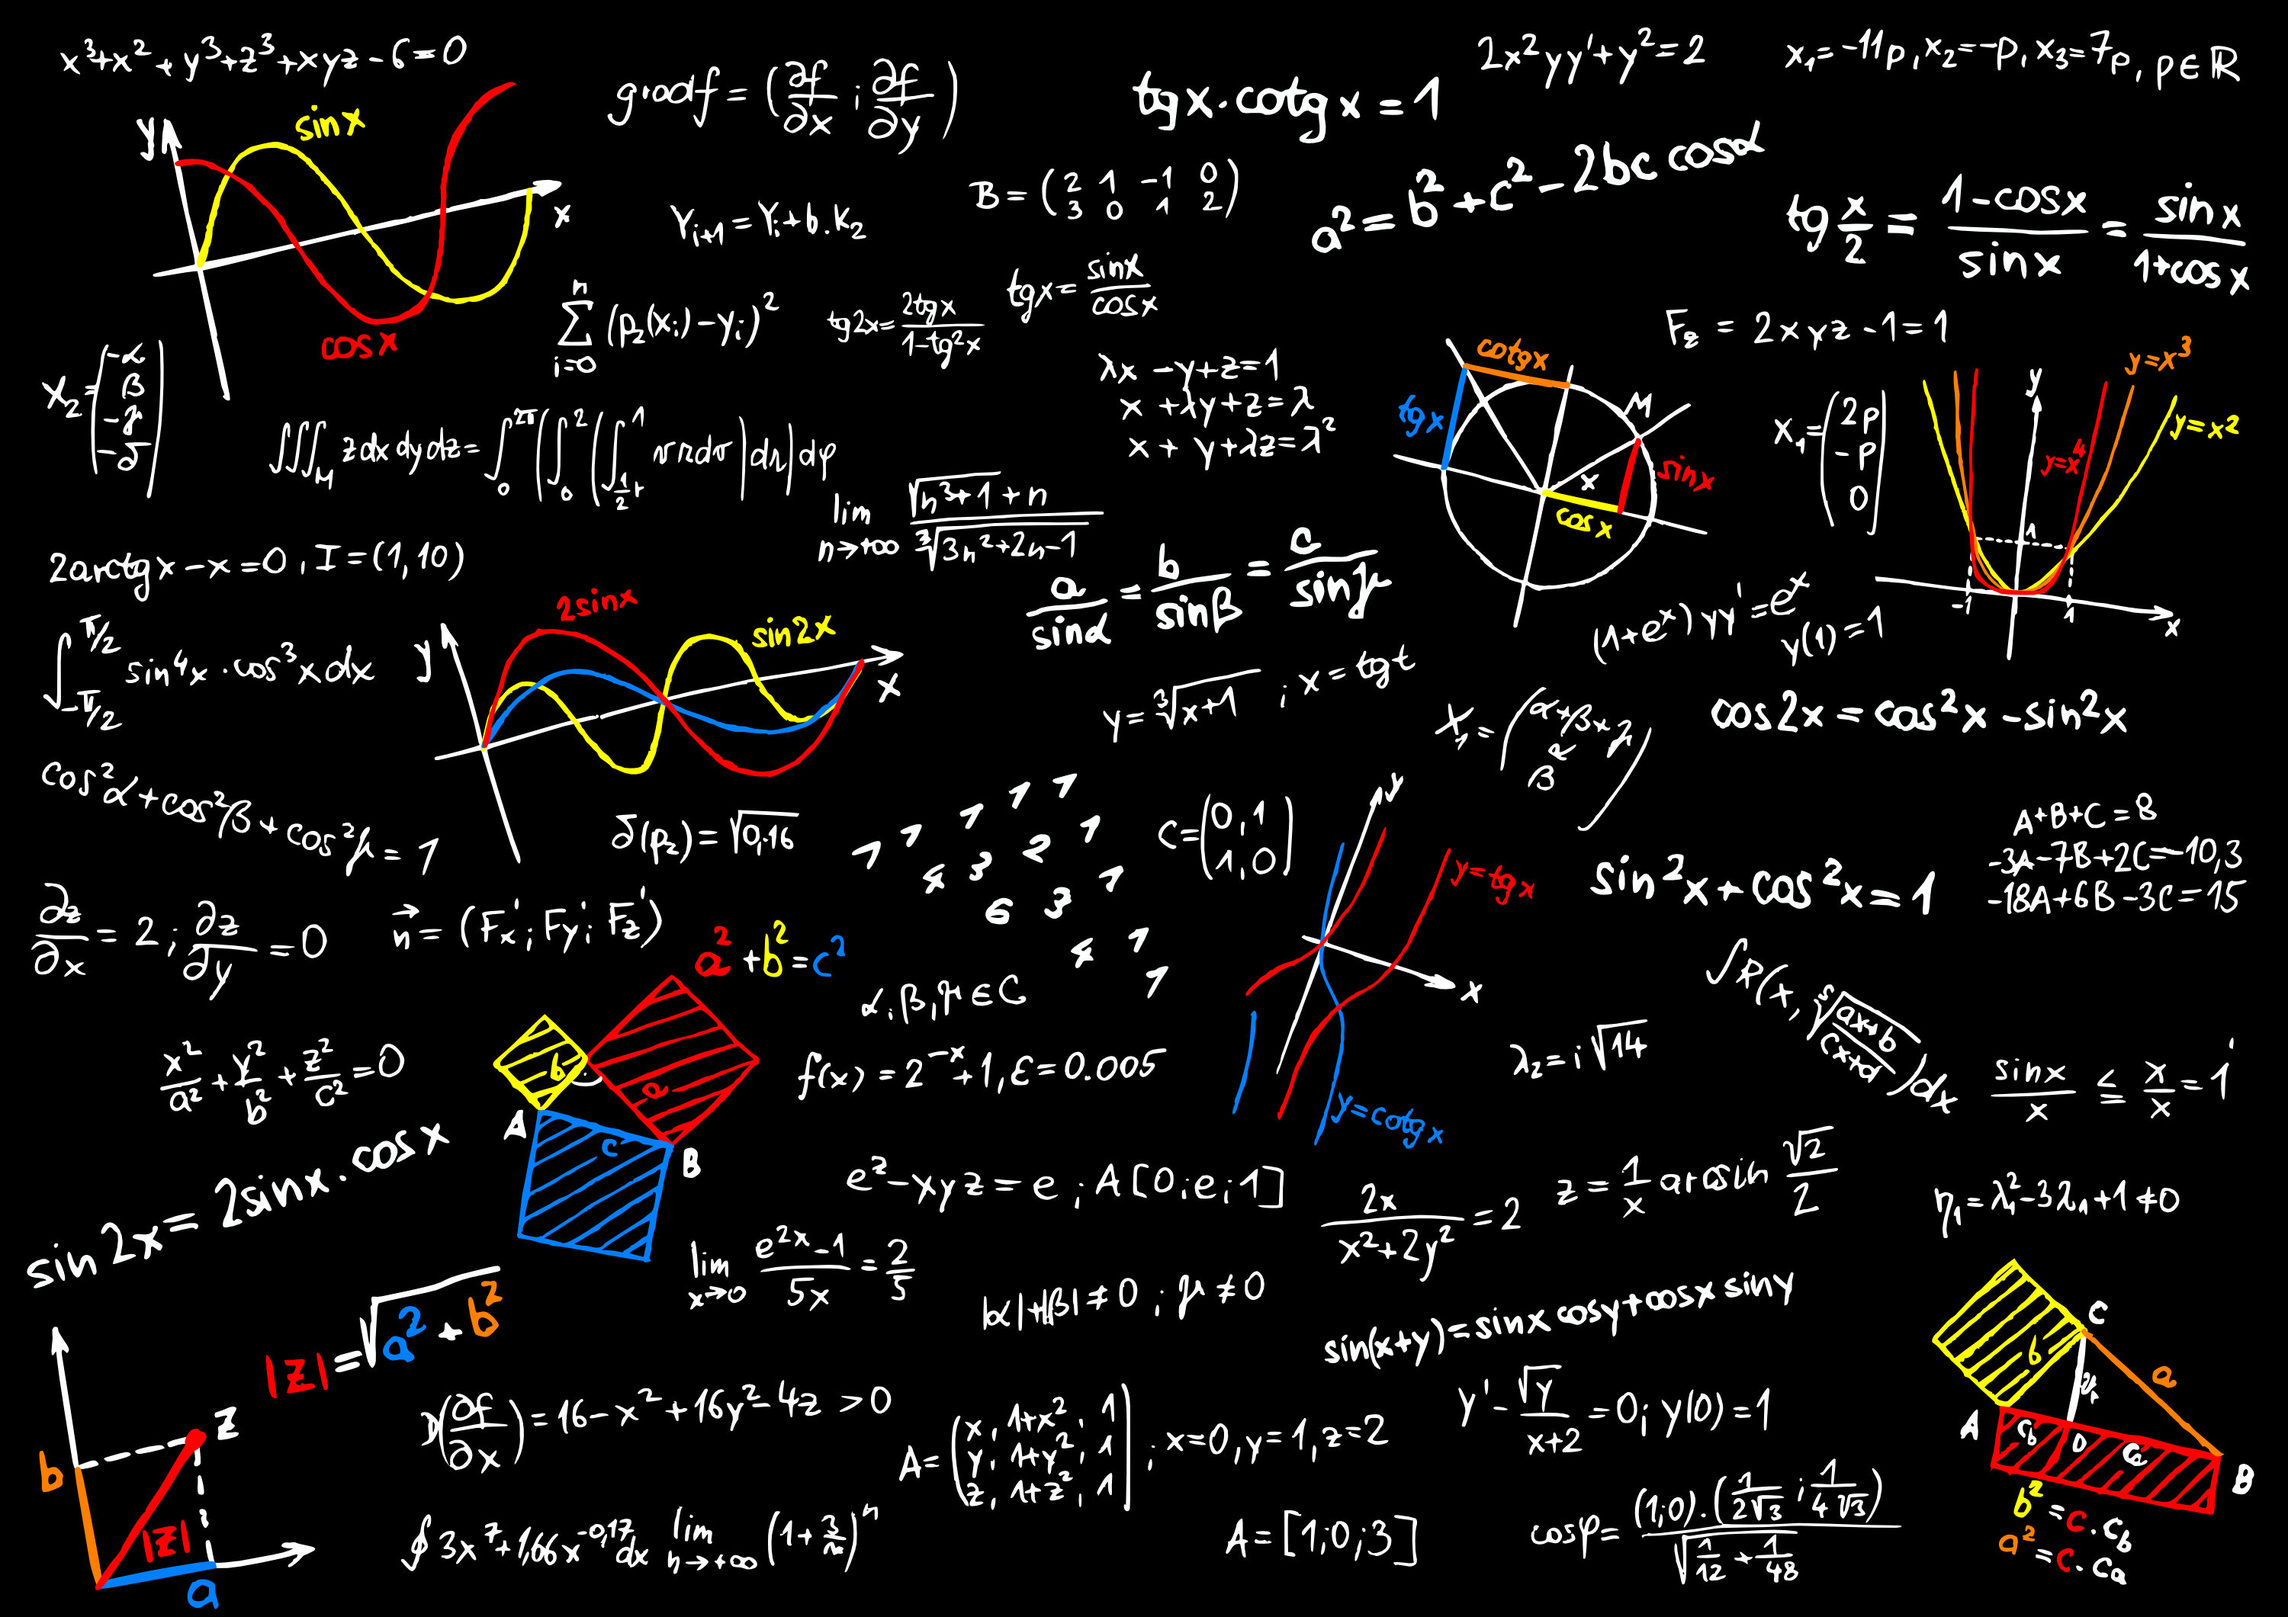
\includegraphics[width=0.3\linewidth]{math}
    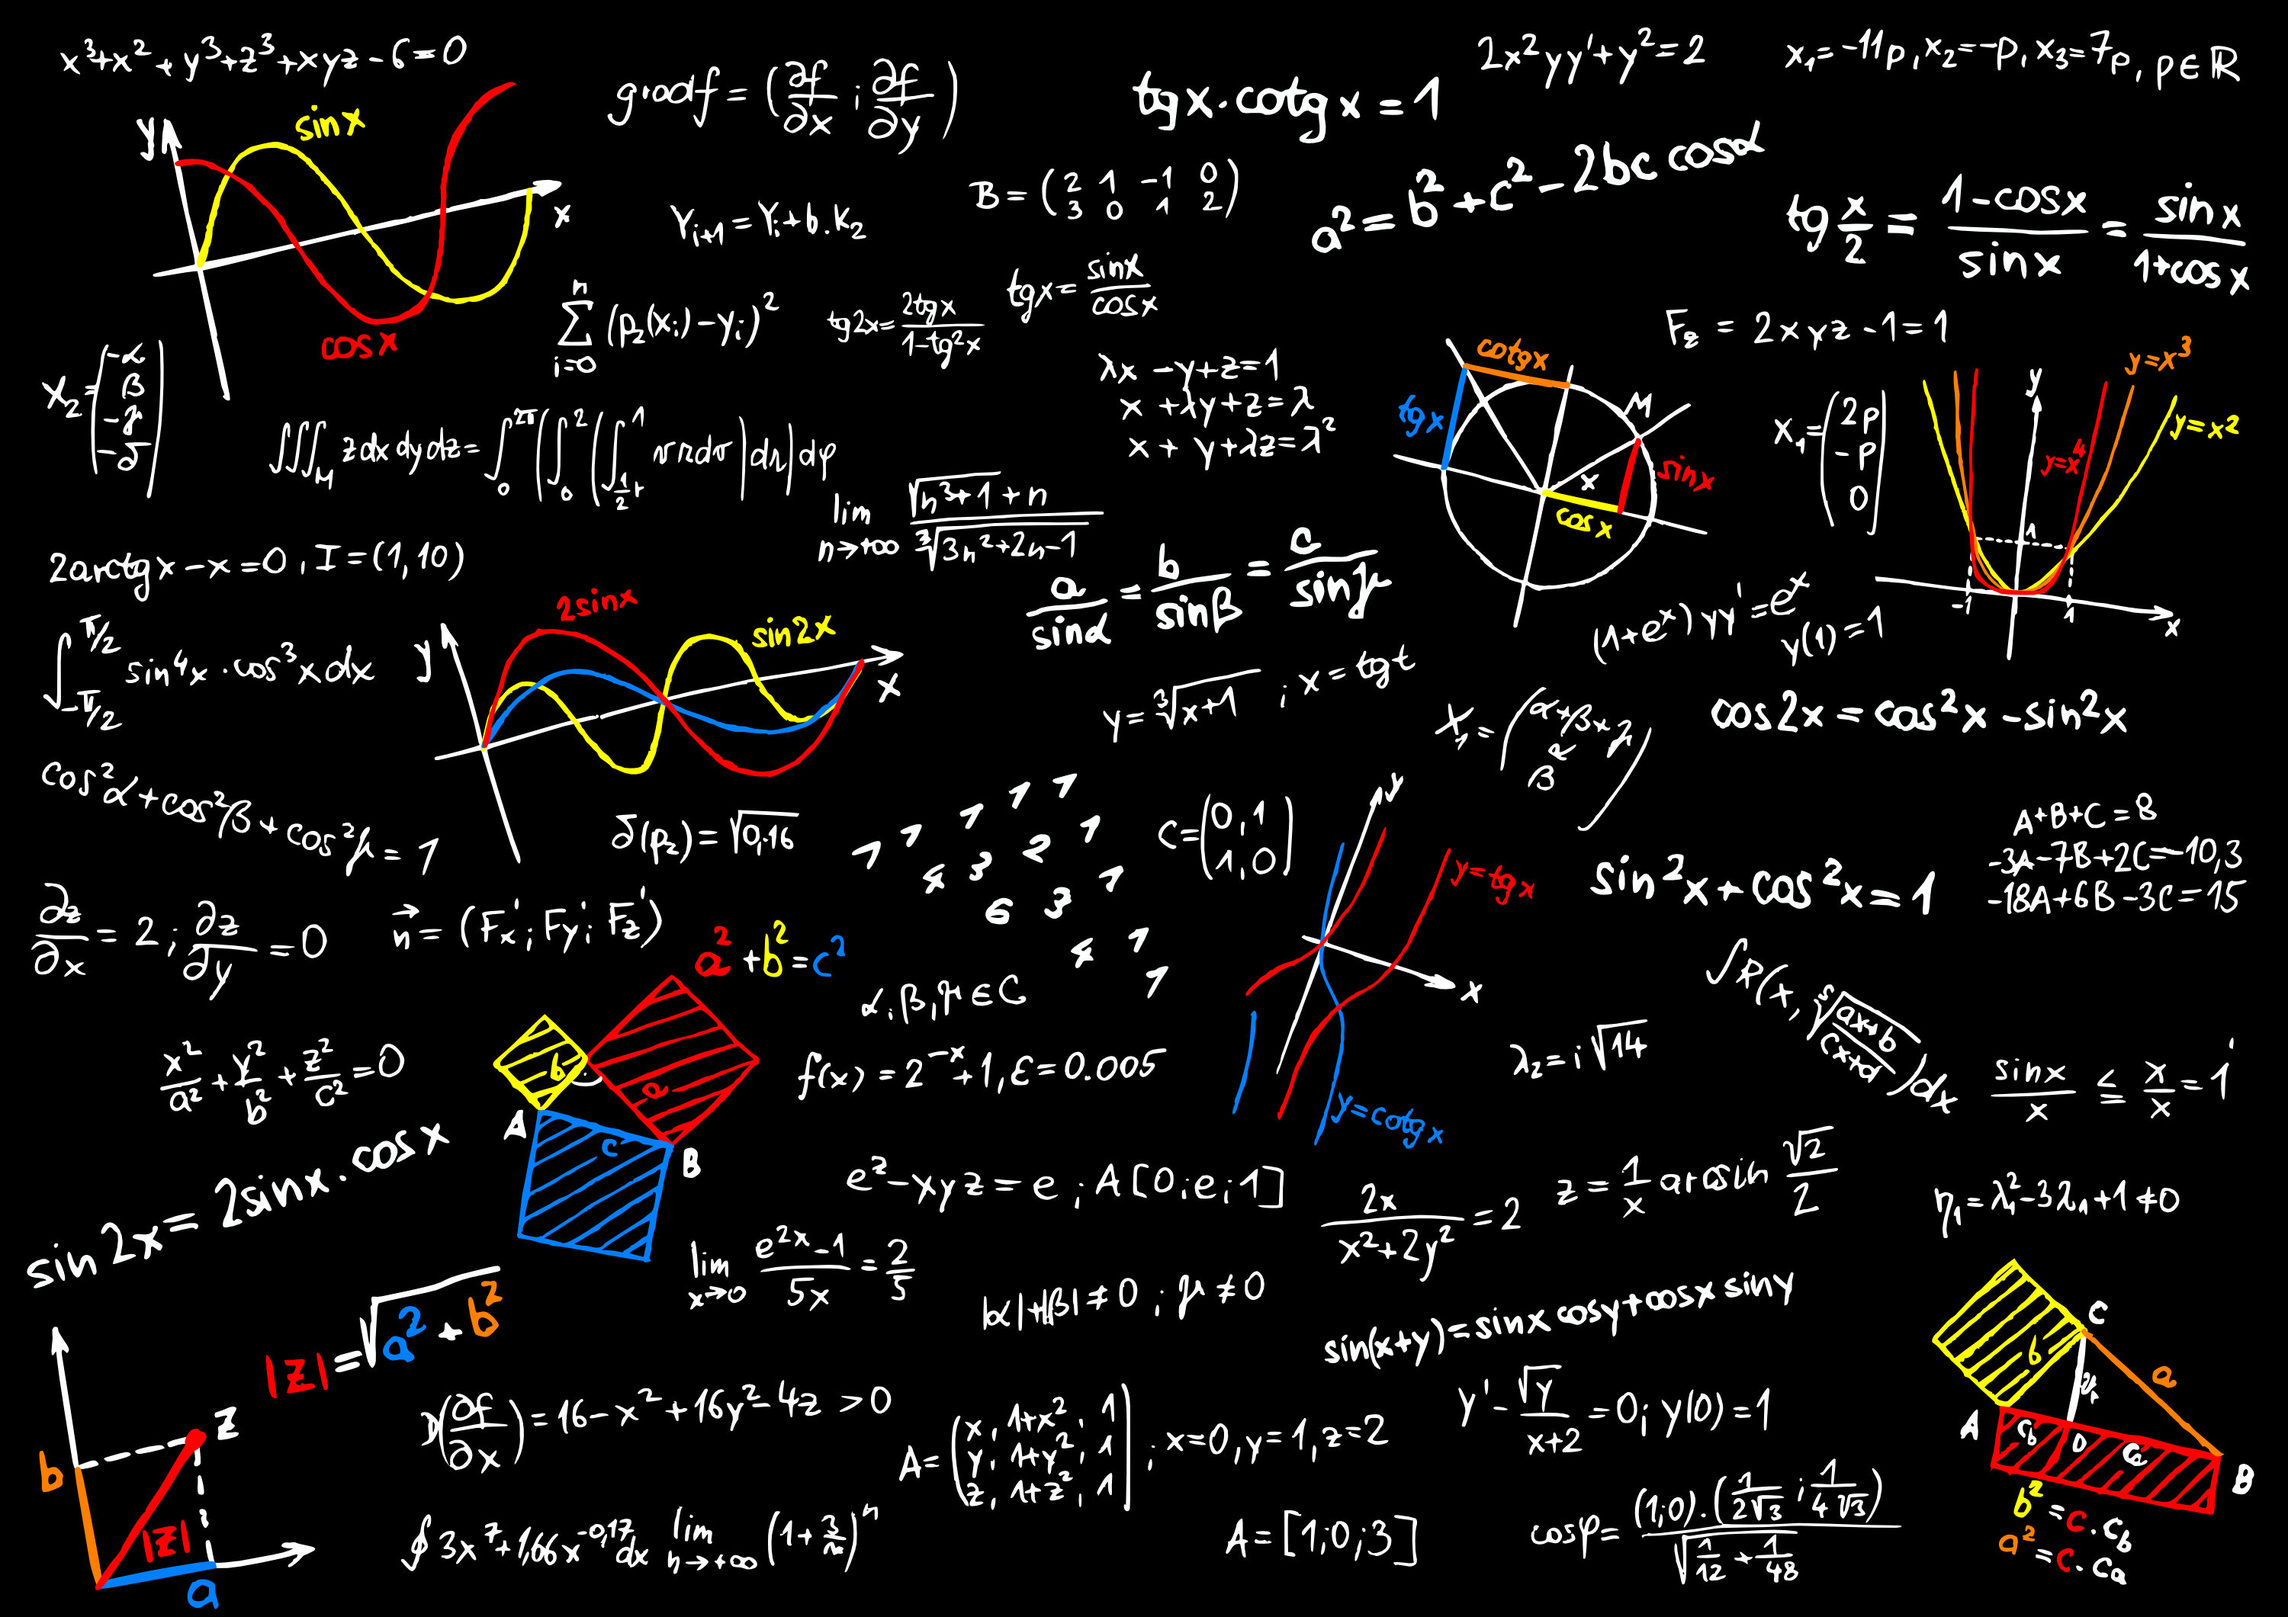
\includegraphics[width=0.1\linewidth]{math}
\end{figure}


% just add \centering before \includegraphics to center the figures
\textbf{2. You can also align figures and center them:}
\begin{figure}[h!]
	\centering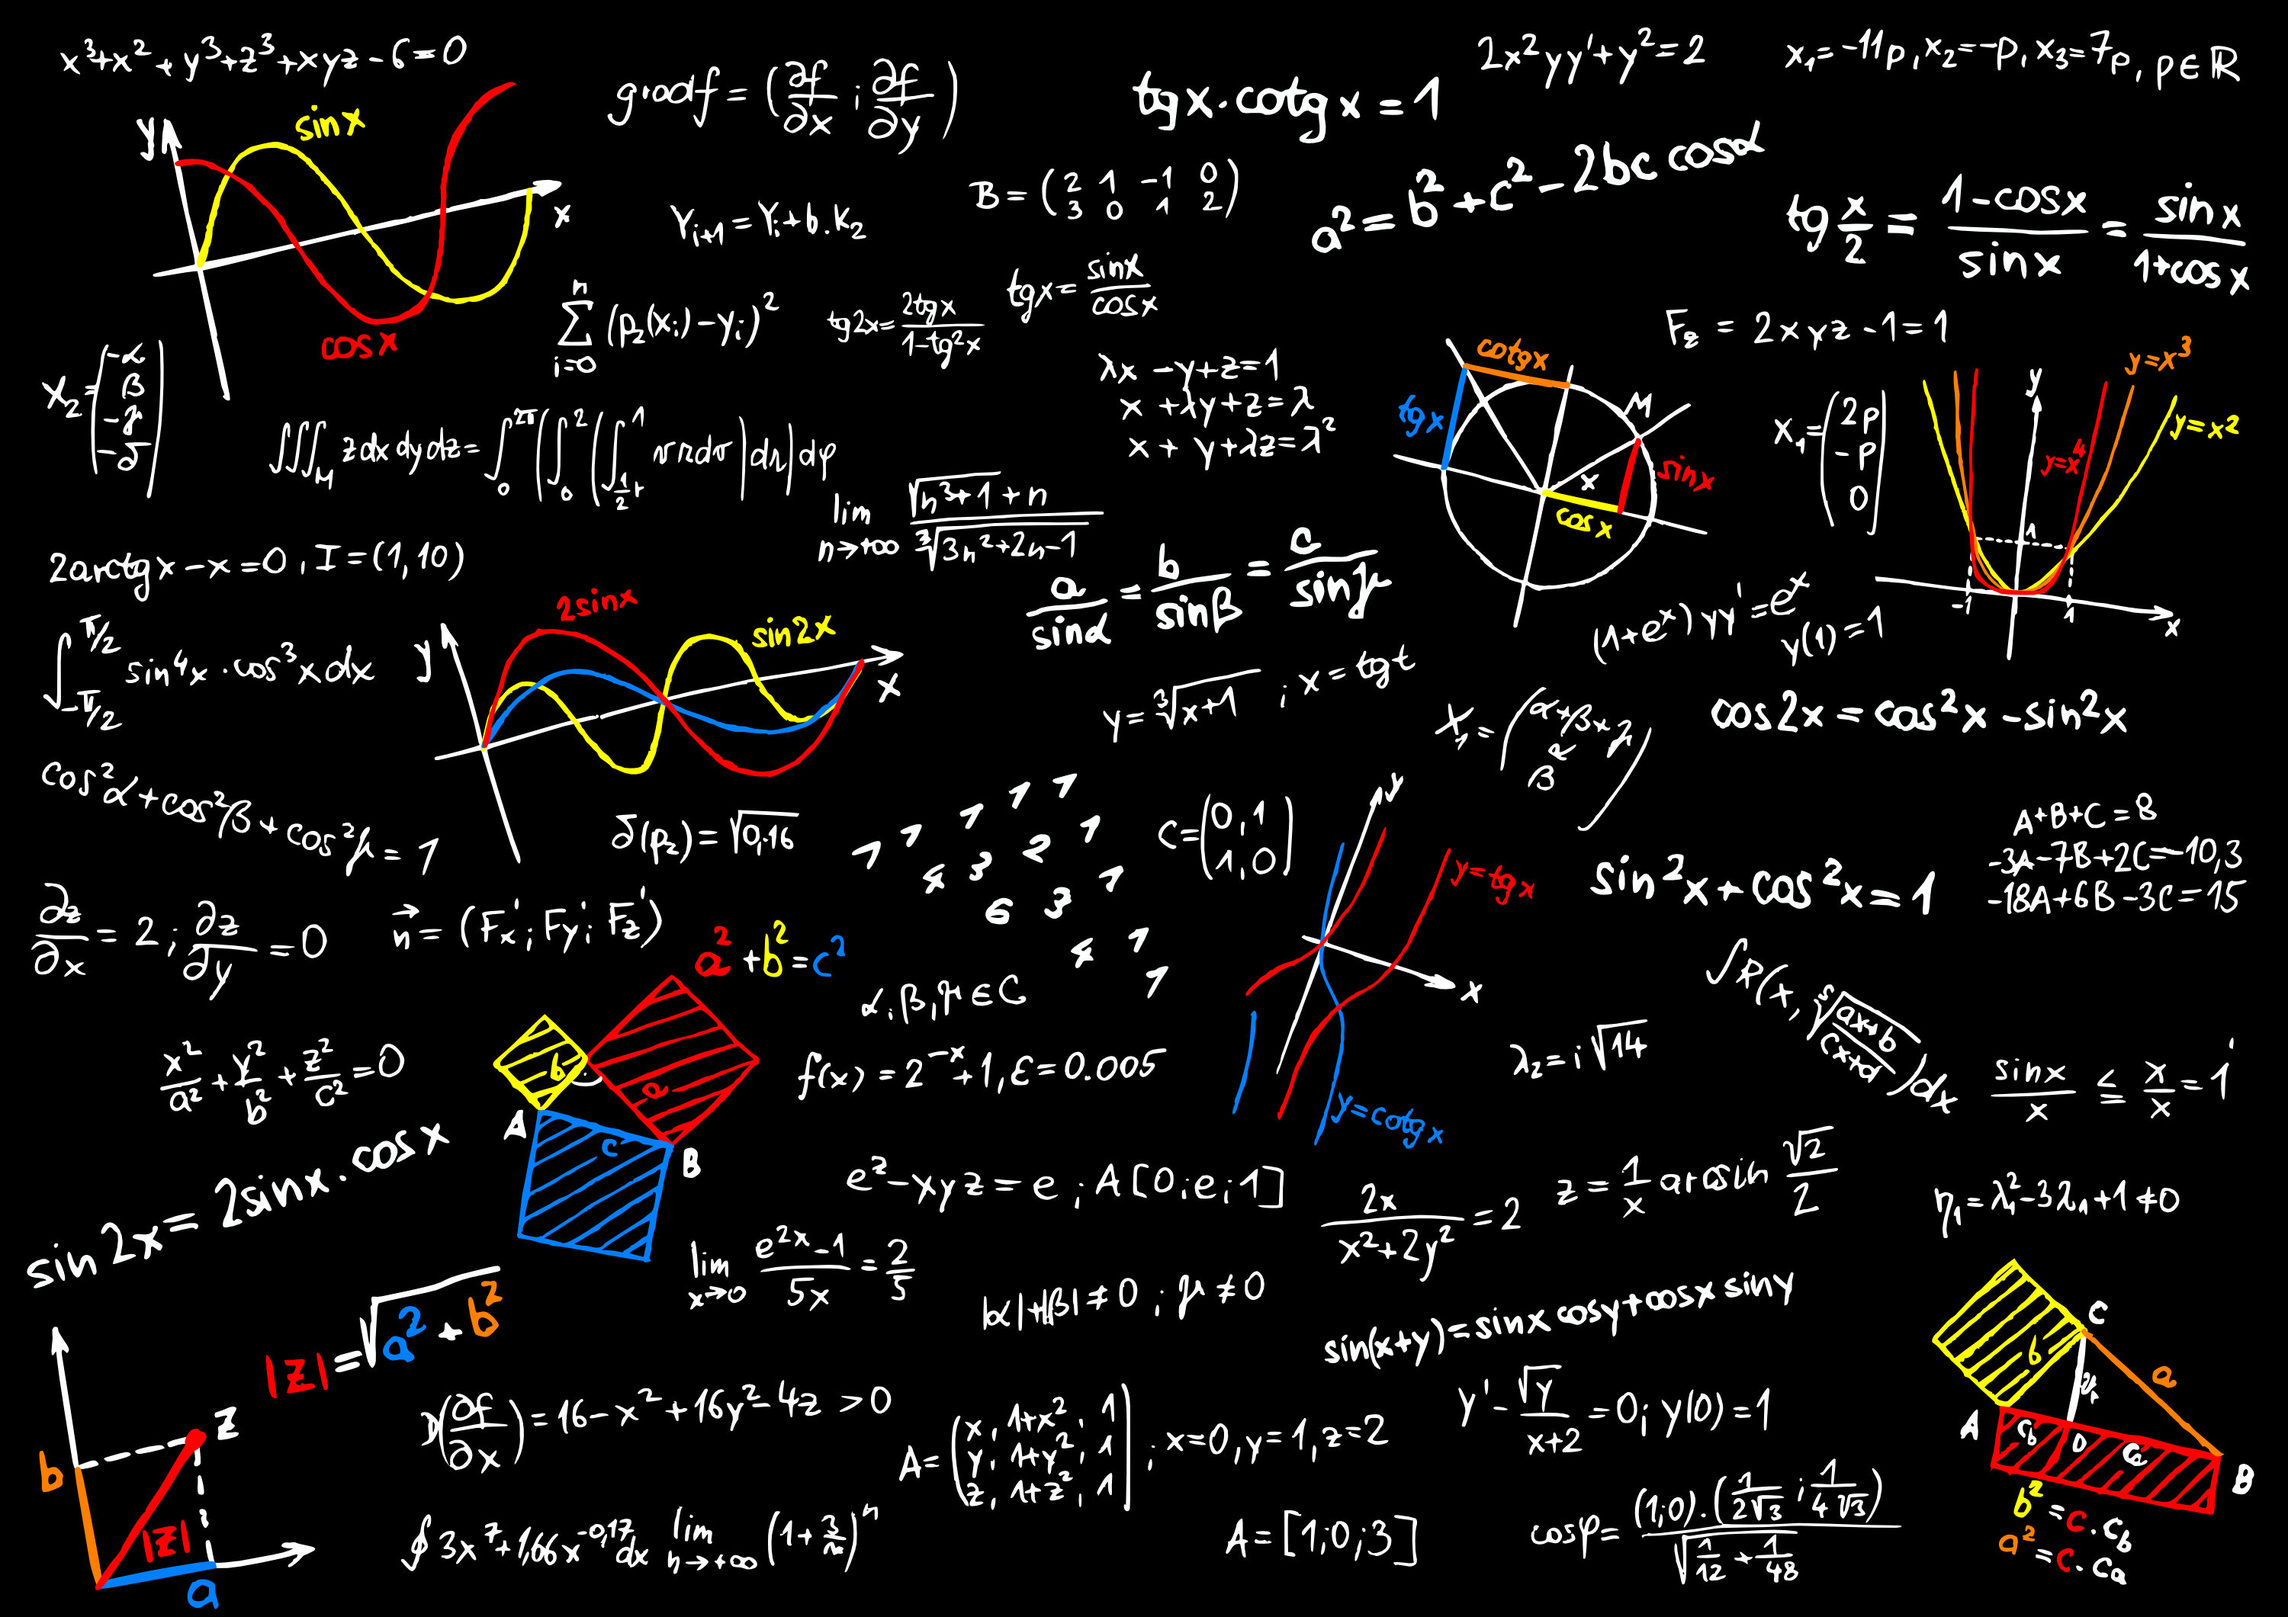
\includegraphics[width=0.3\linewidth]{math}
    \centering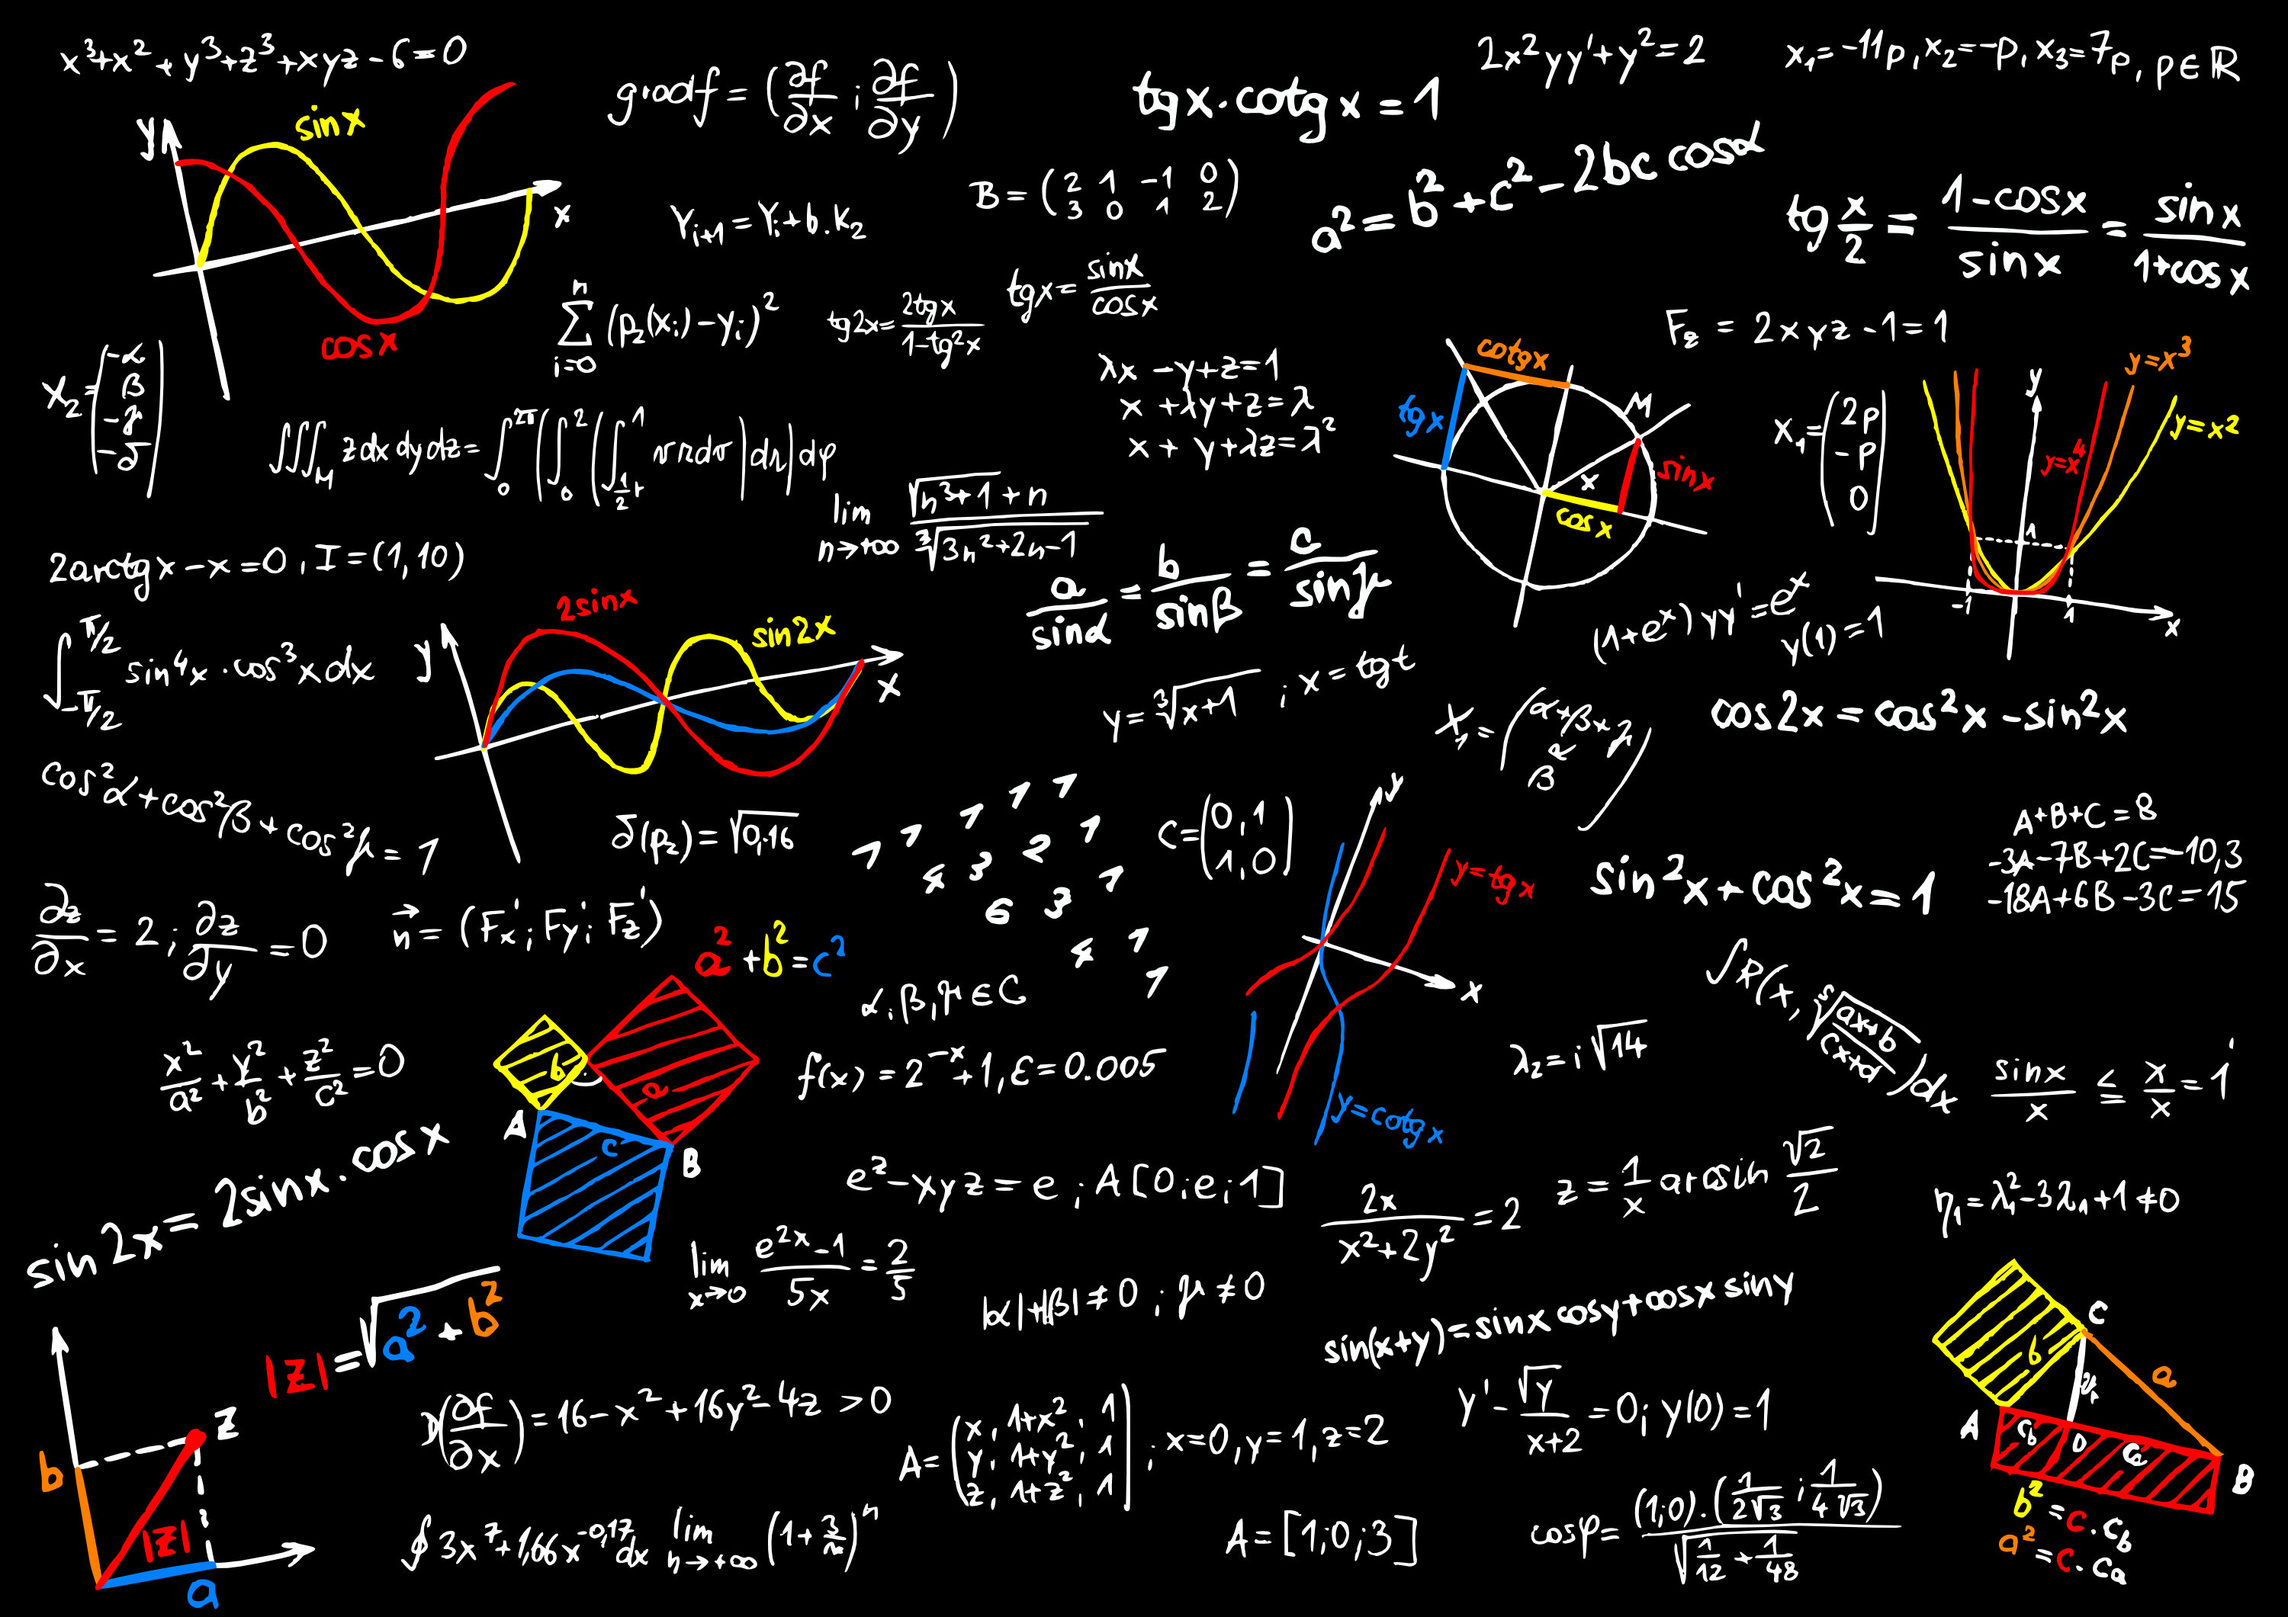
\includegraphics[width=0.2\linewidth]{math}
\end{figure}

\textbf{3. And you can add captions and figure numbers}

\begin{figure}[h!] % the [h!] aligns the figure to top of the current section/space
	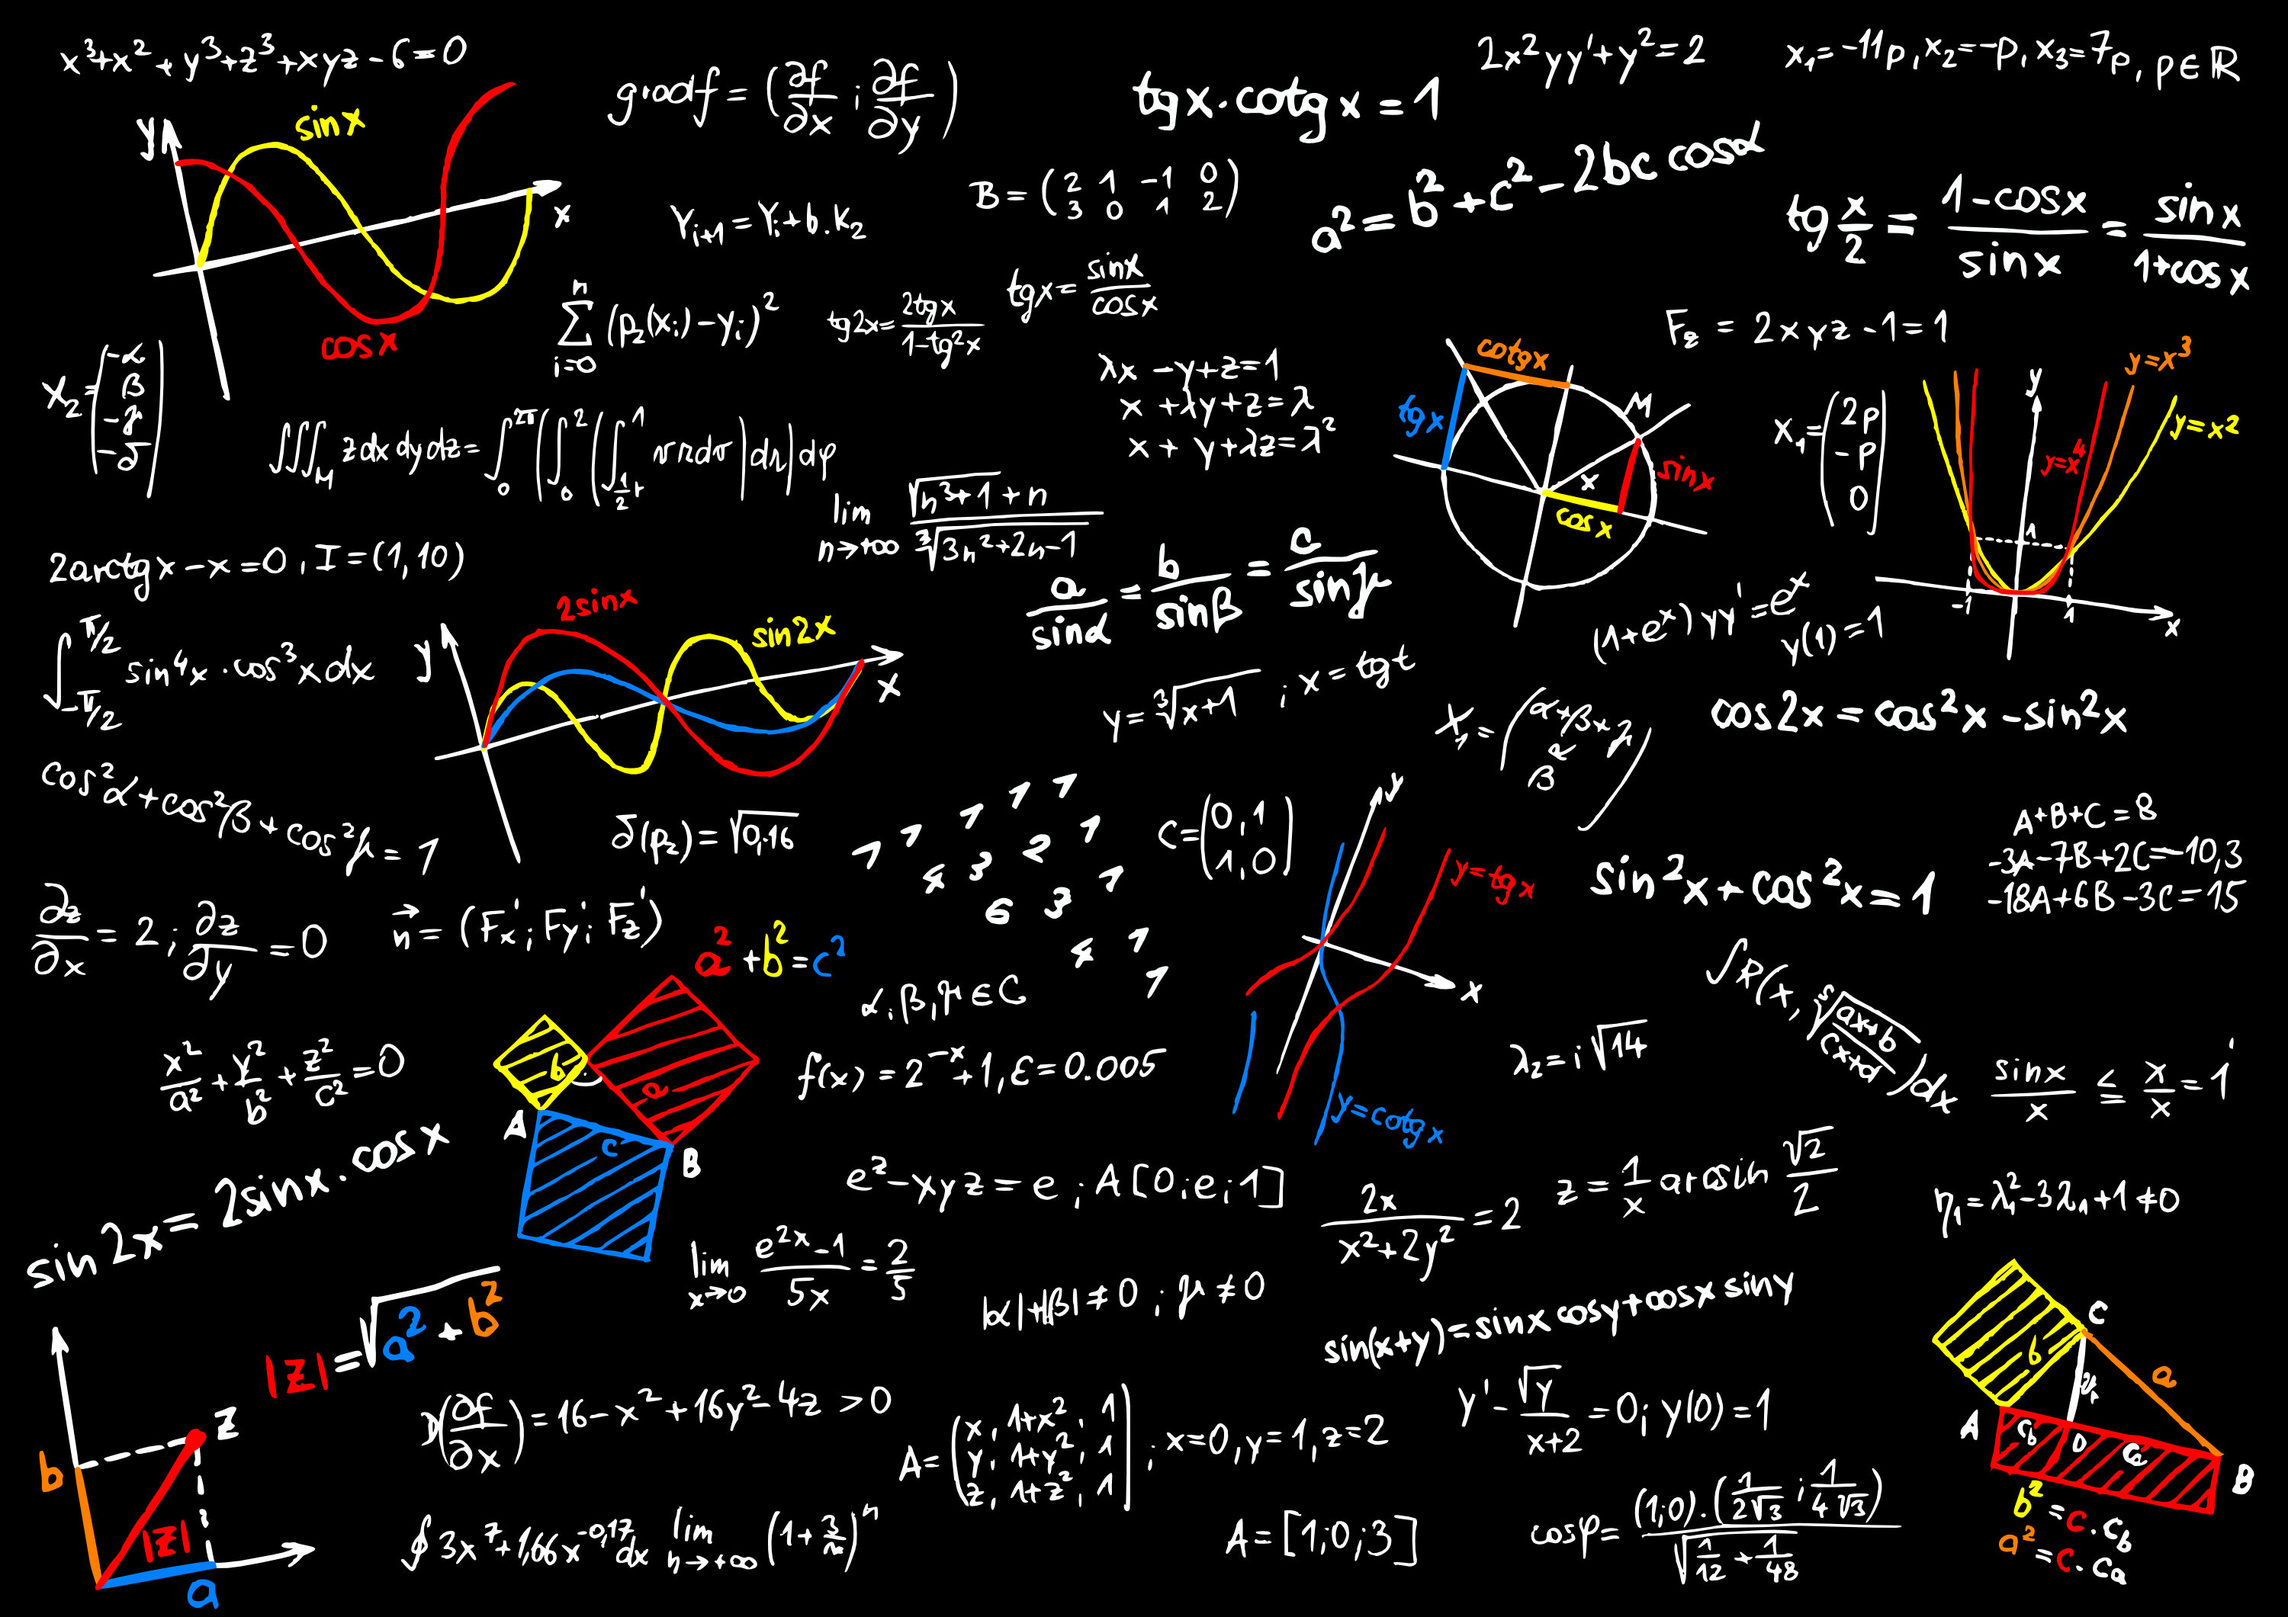
\includegraphics[width=0.3\linewidth]{math}    
    \caption{Caption on Bottom}
\end{figure}
   
% Multiple figure captions
\newpage
\textbf{4. Captions for multiple images}
\begin{figure}[h!]
    \label{fig:figlabel}
    \begin{center}
      \subfloat[Subcaption a]      {
      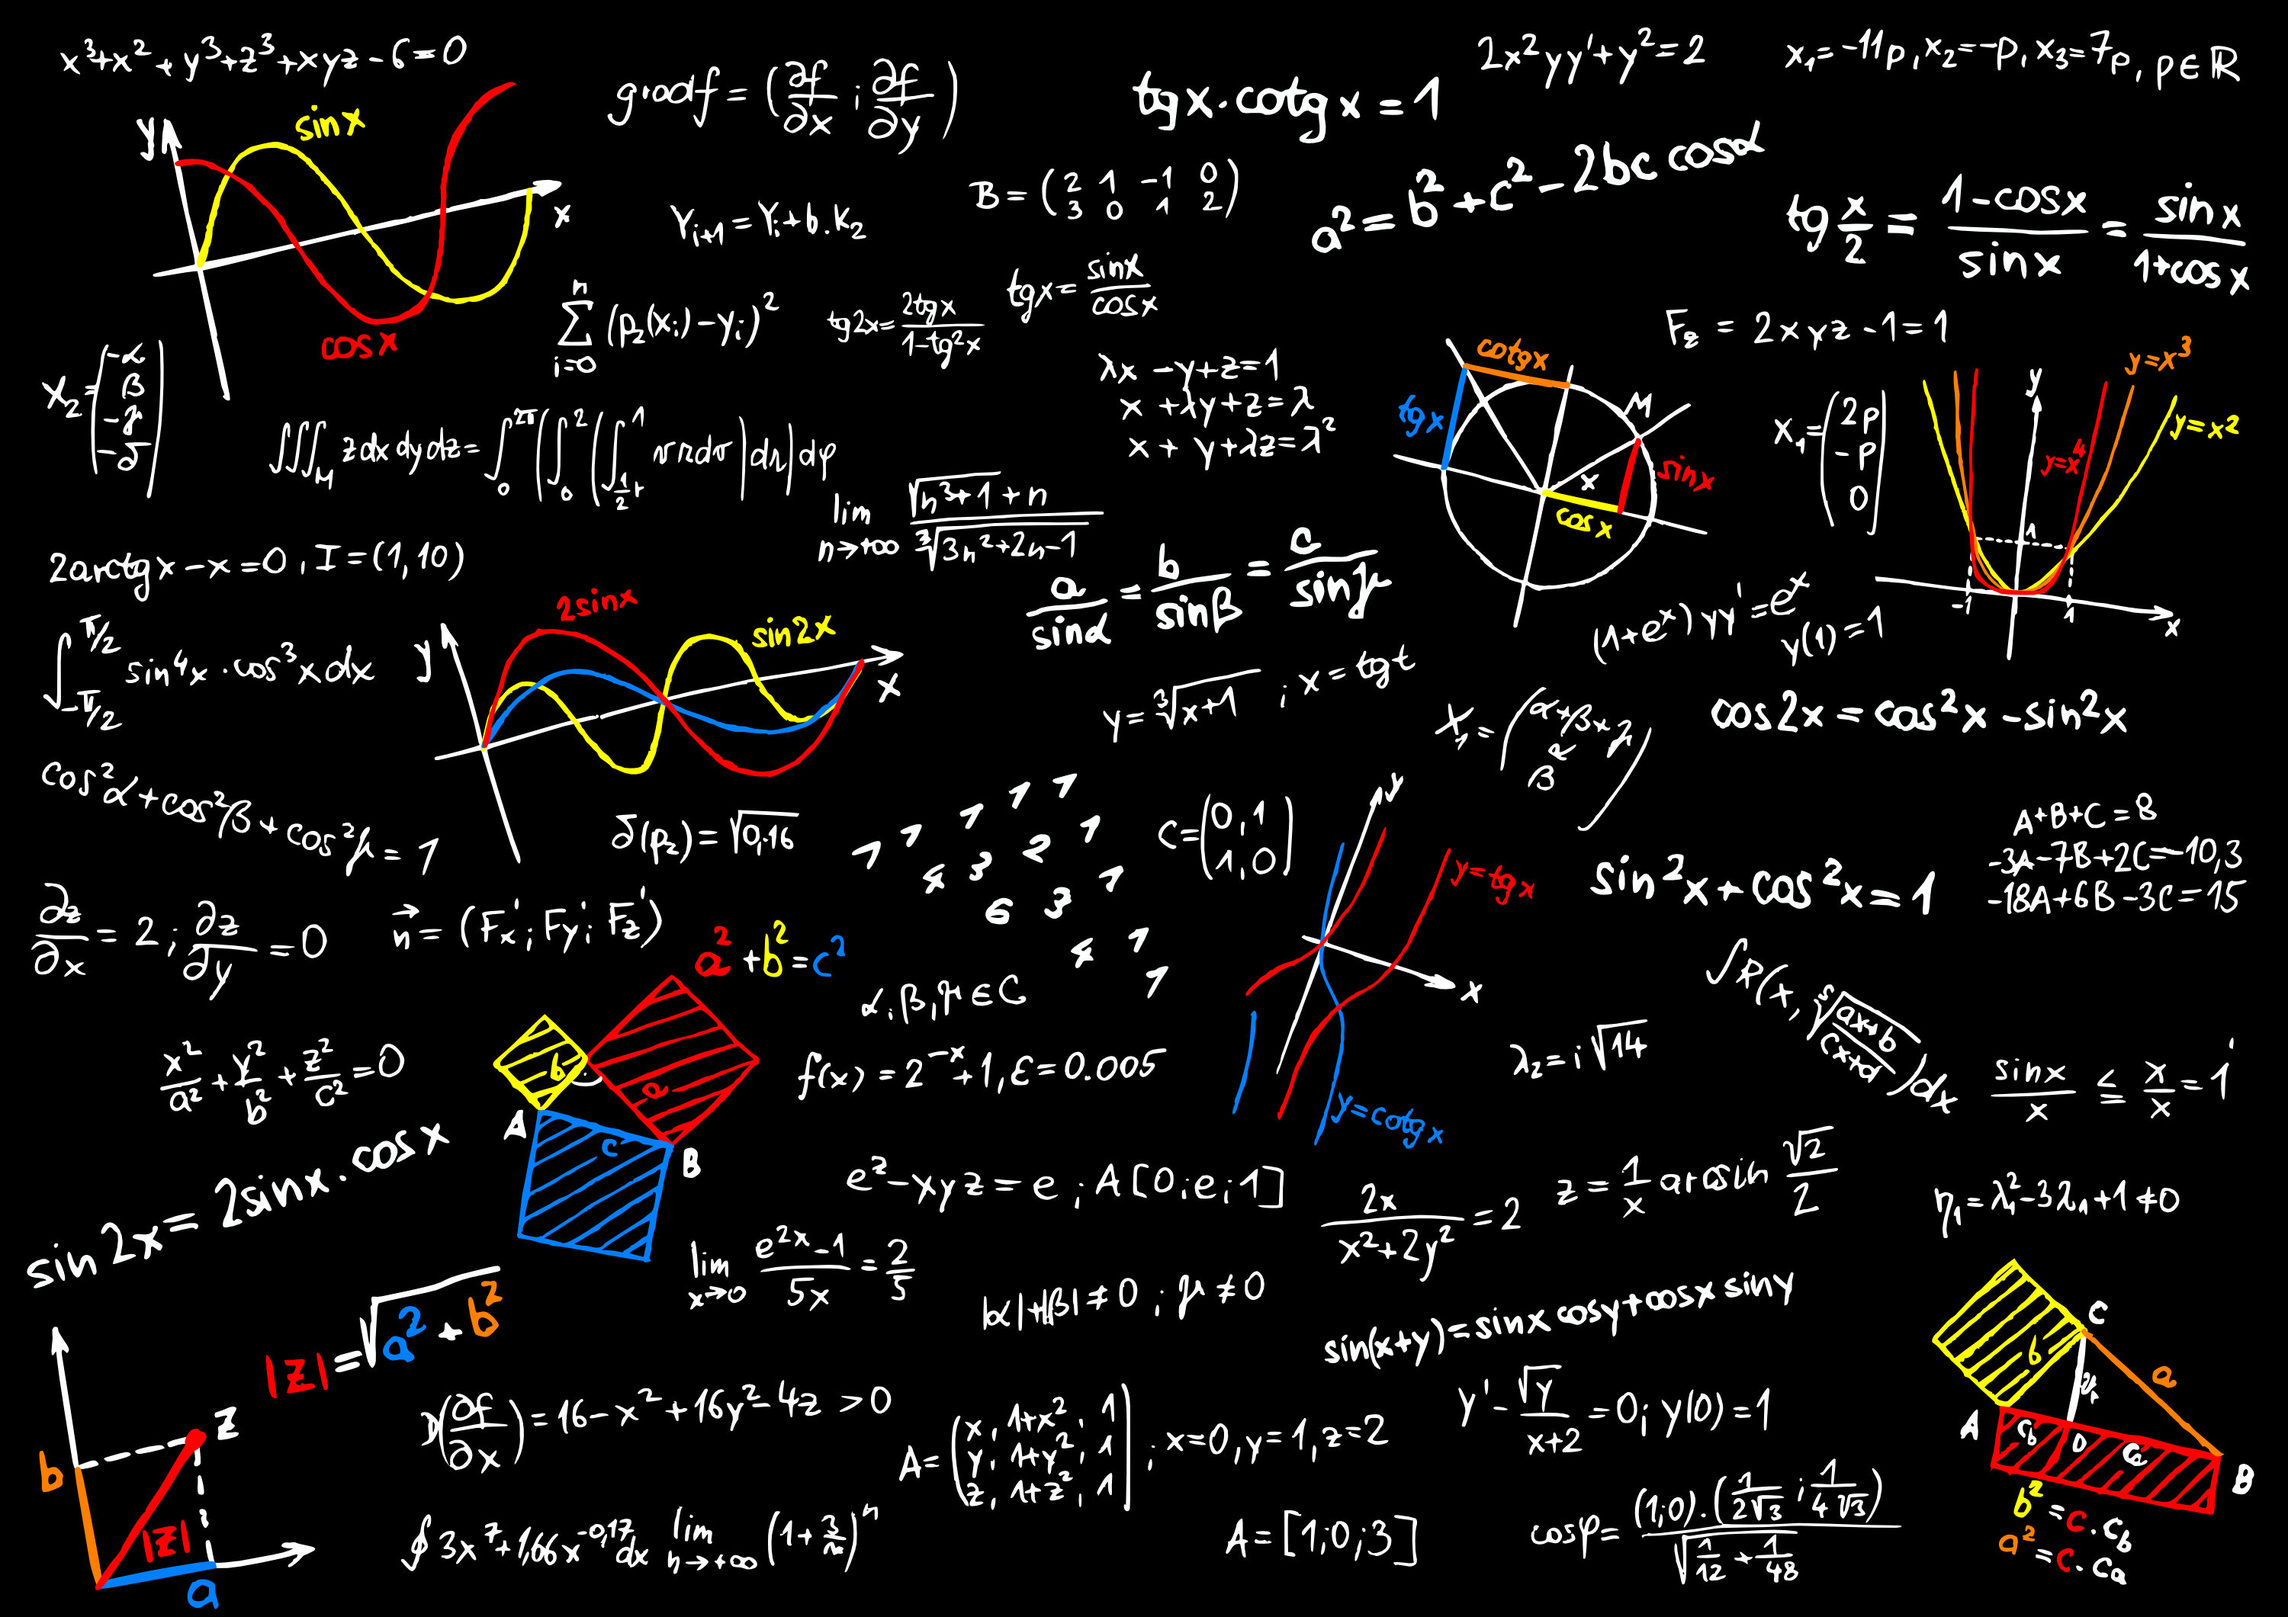
\includegraphics[width=.45\linewidth]{math}
      }\quad
      \subfloat[Subcaption b]      {
      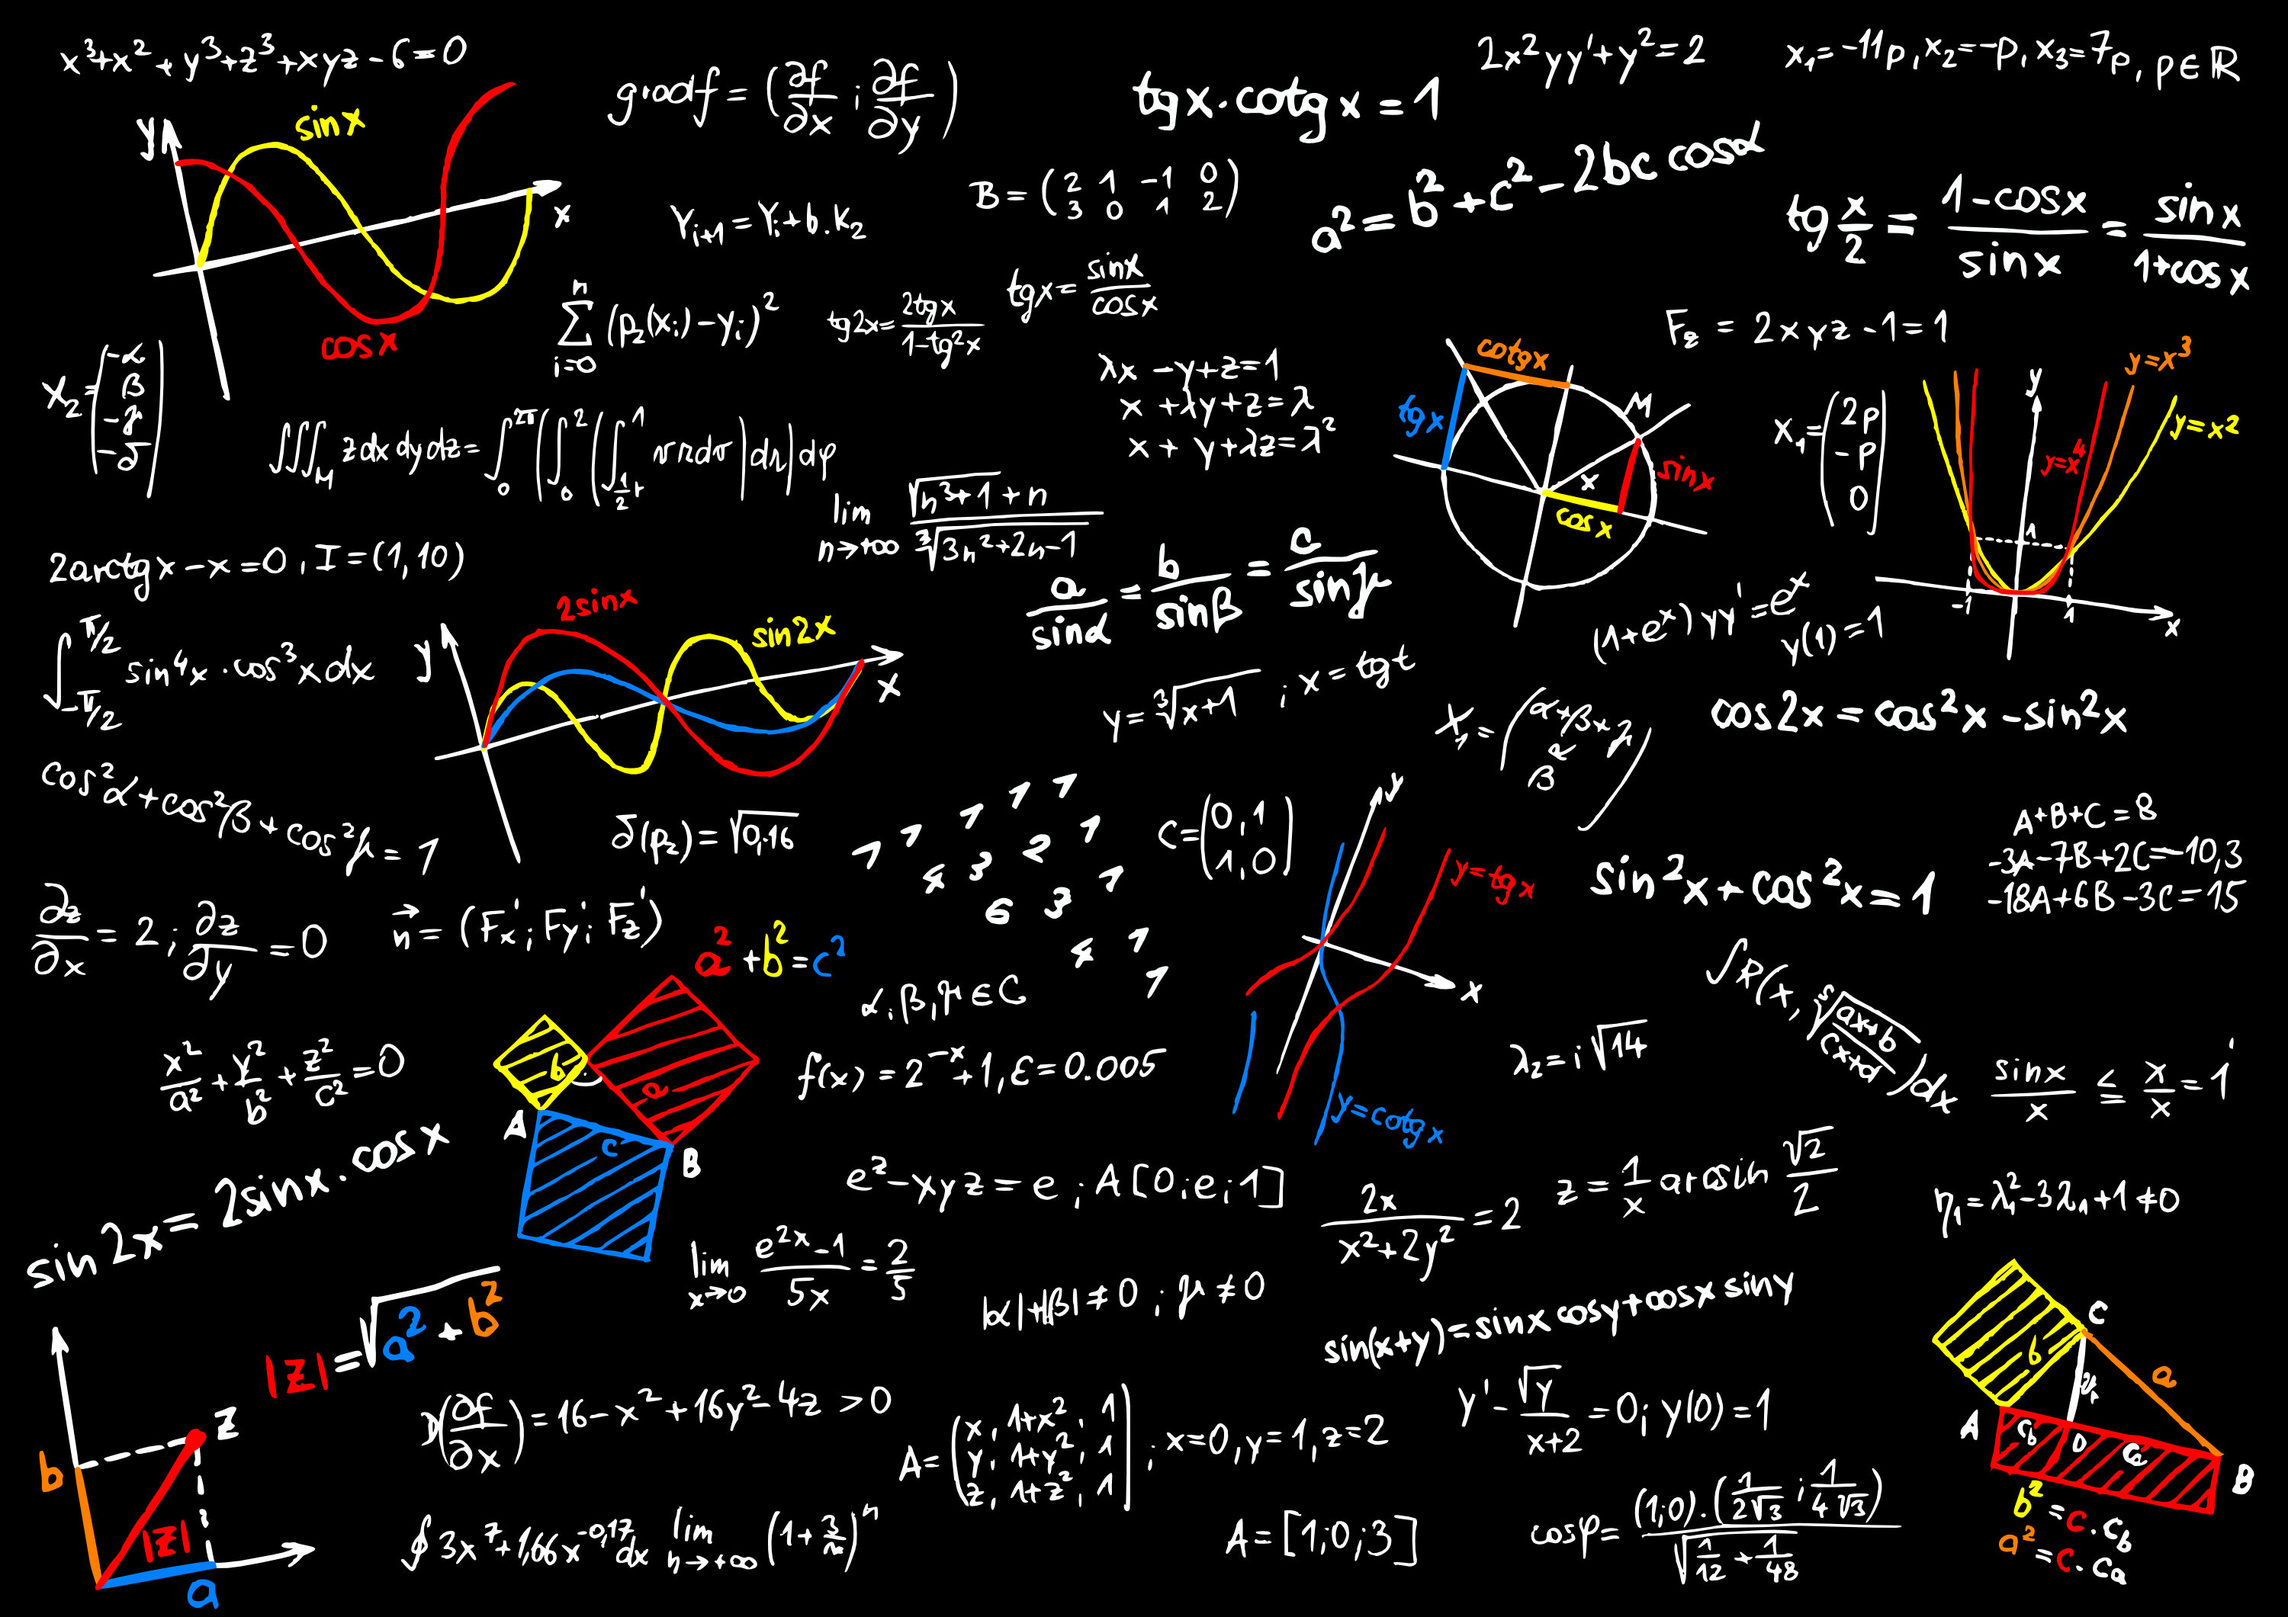
\includegraphics[width=.45\linewidth]{math}
      }\\
      \subfloat[Subcaption c]      {
      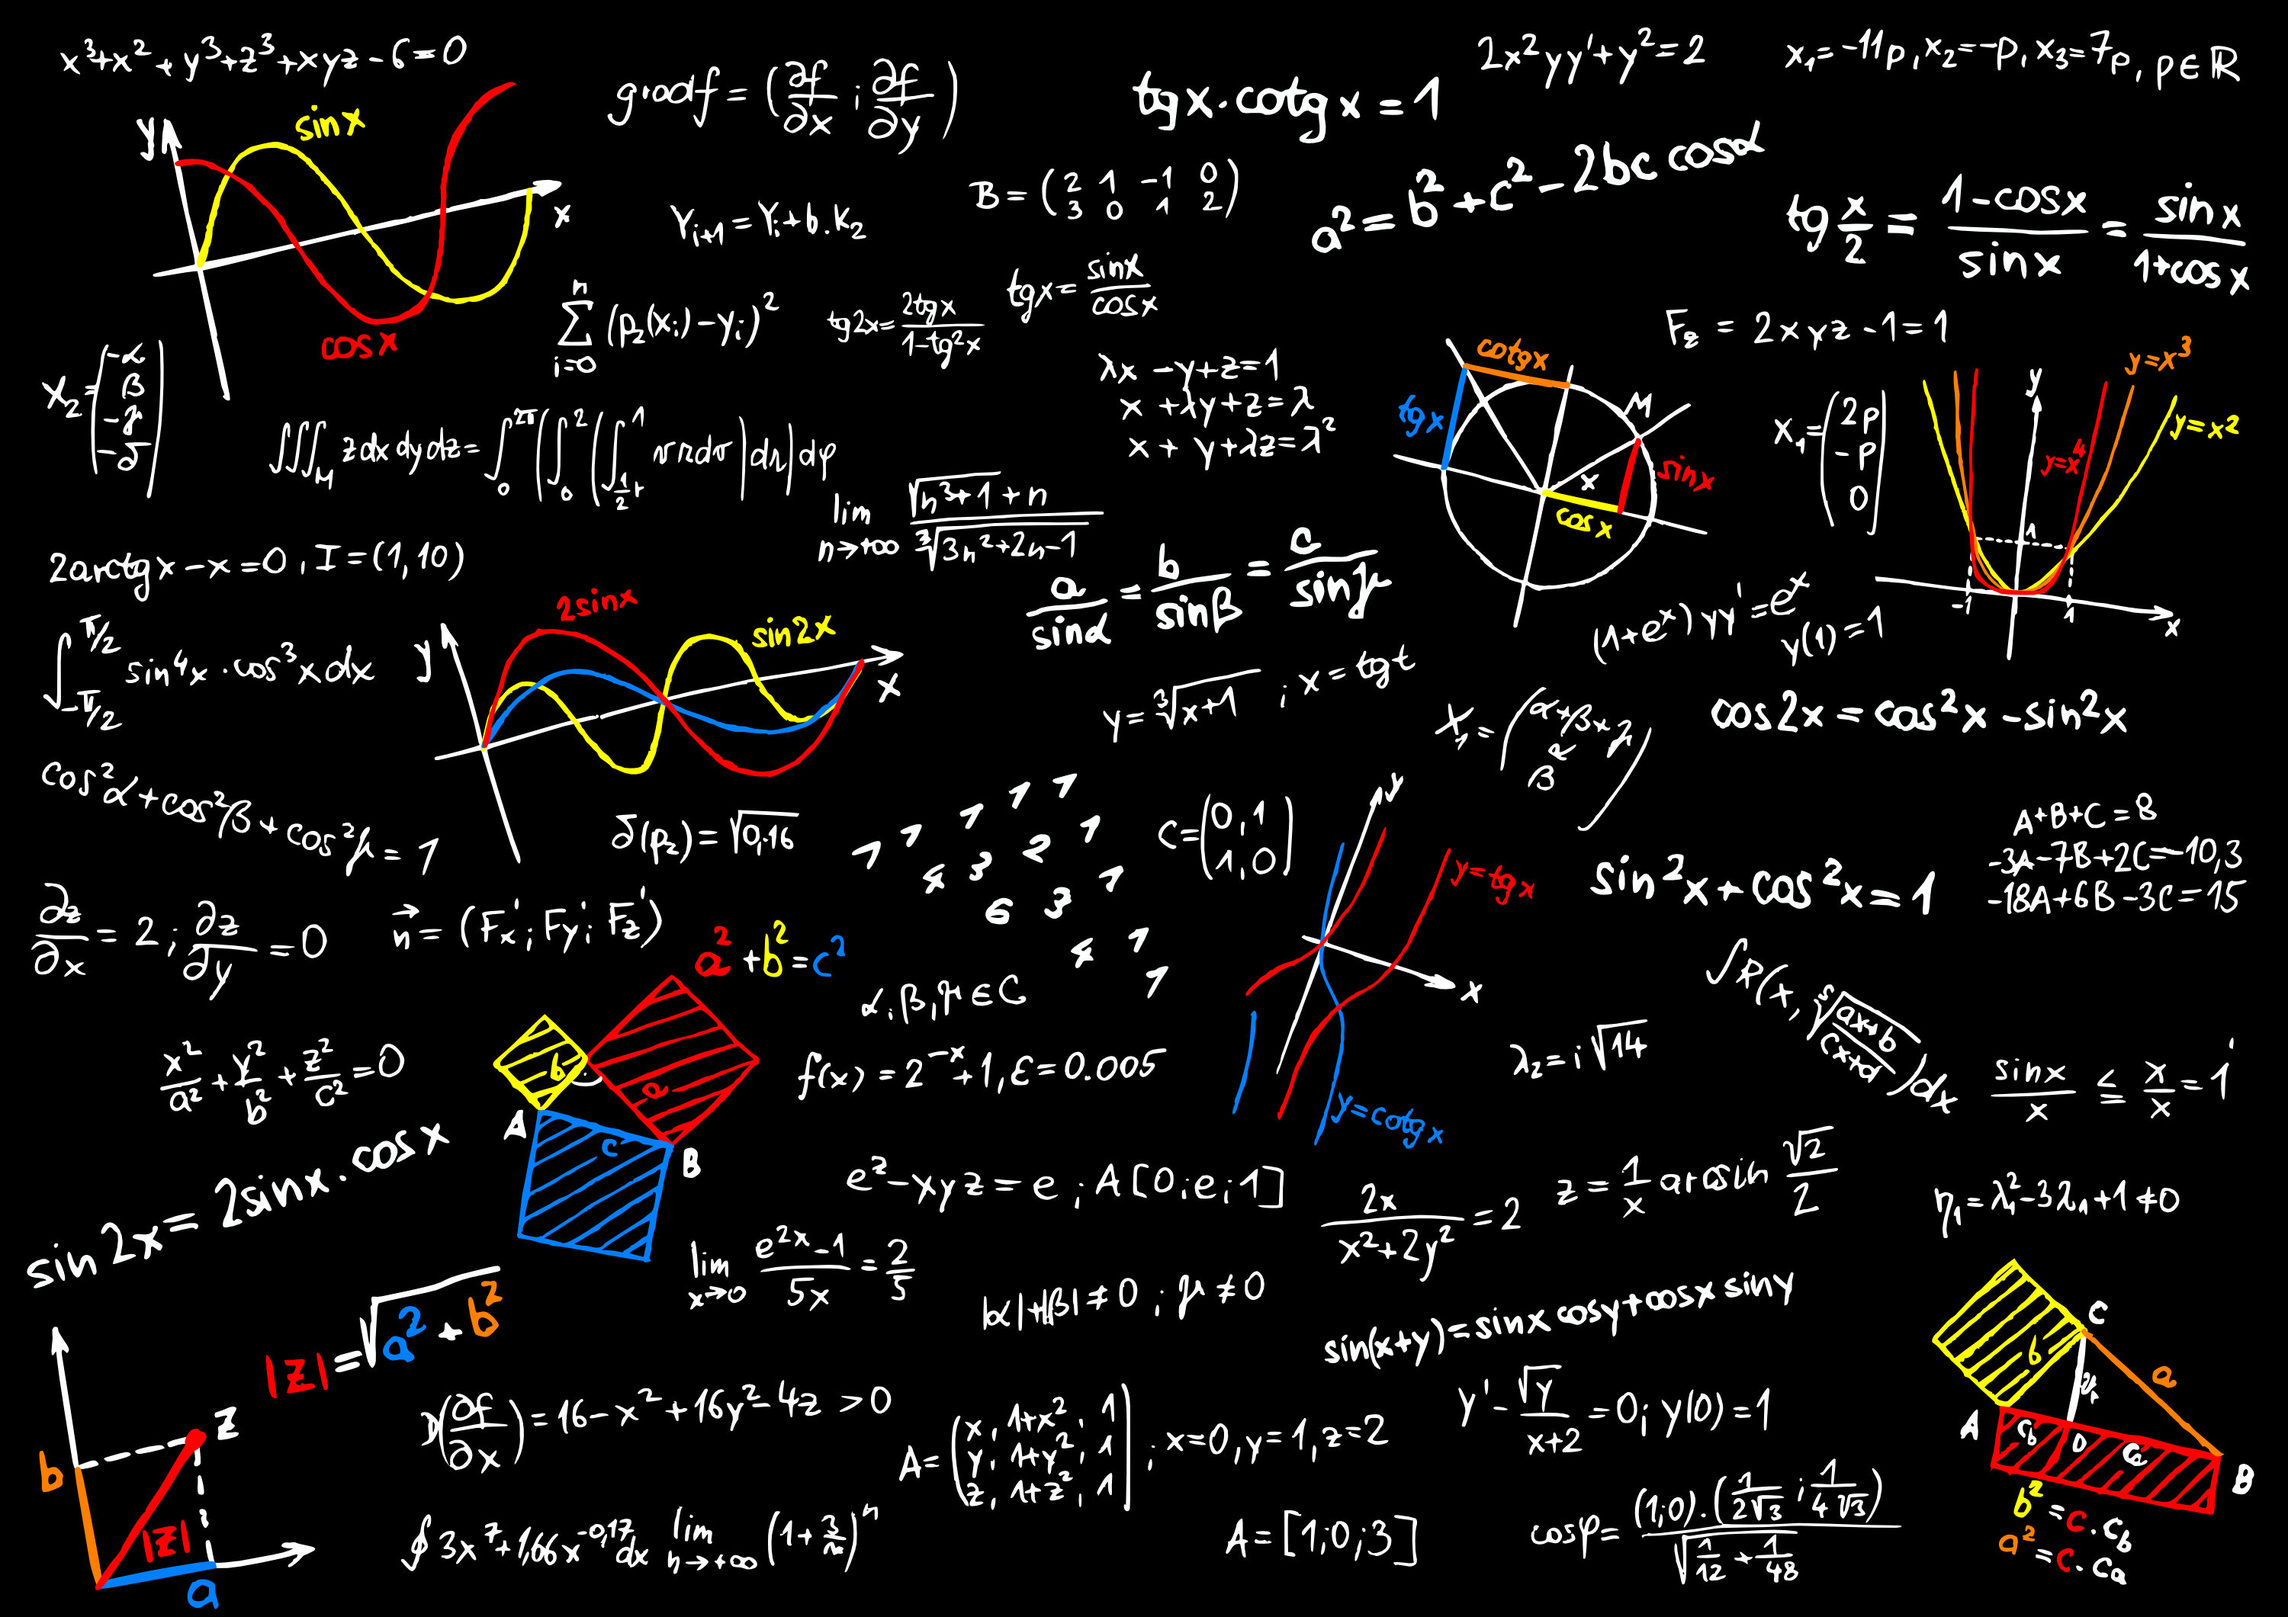
\includegraphics[width=.45\linewidth]{math}
      }\quad
      \subfloat[Subcaption d]      {
      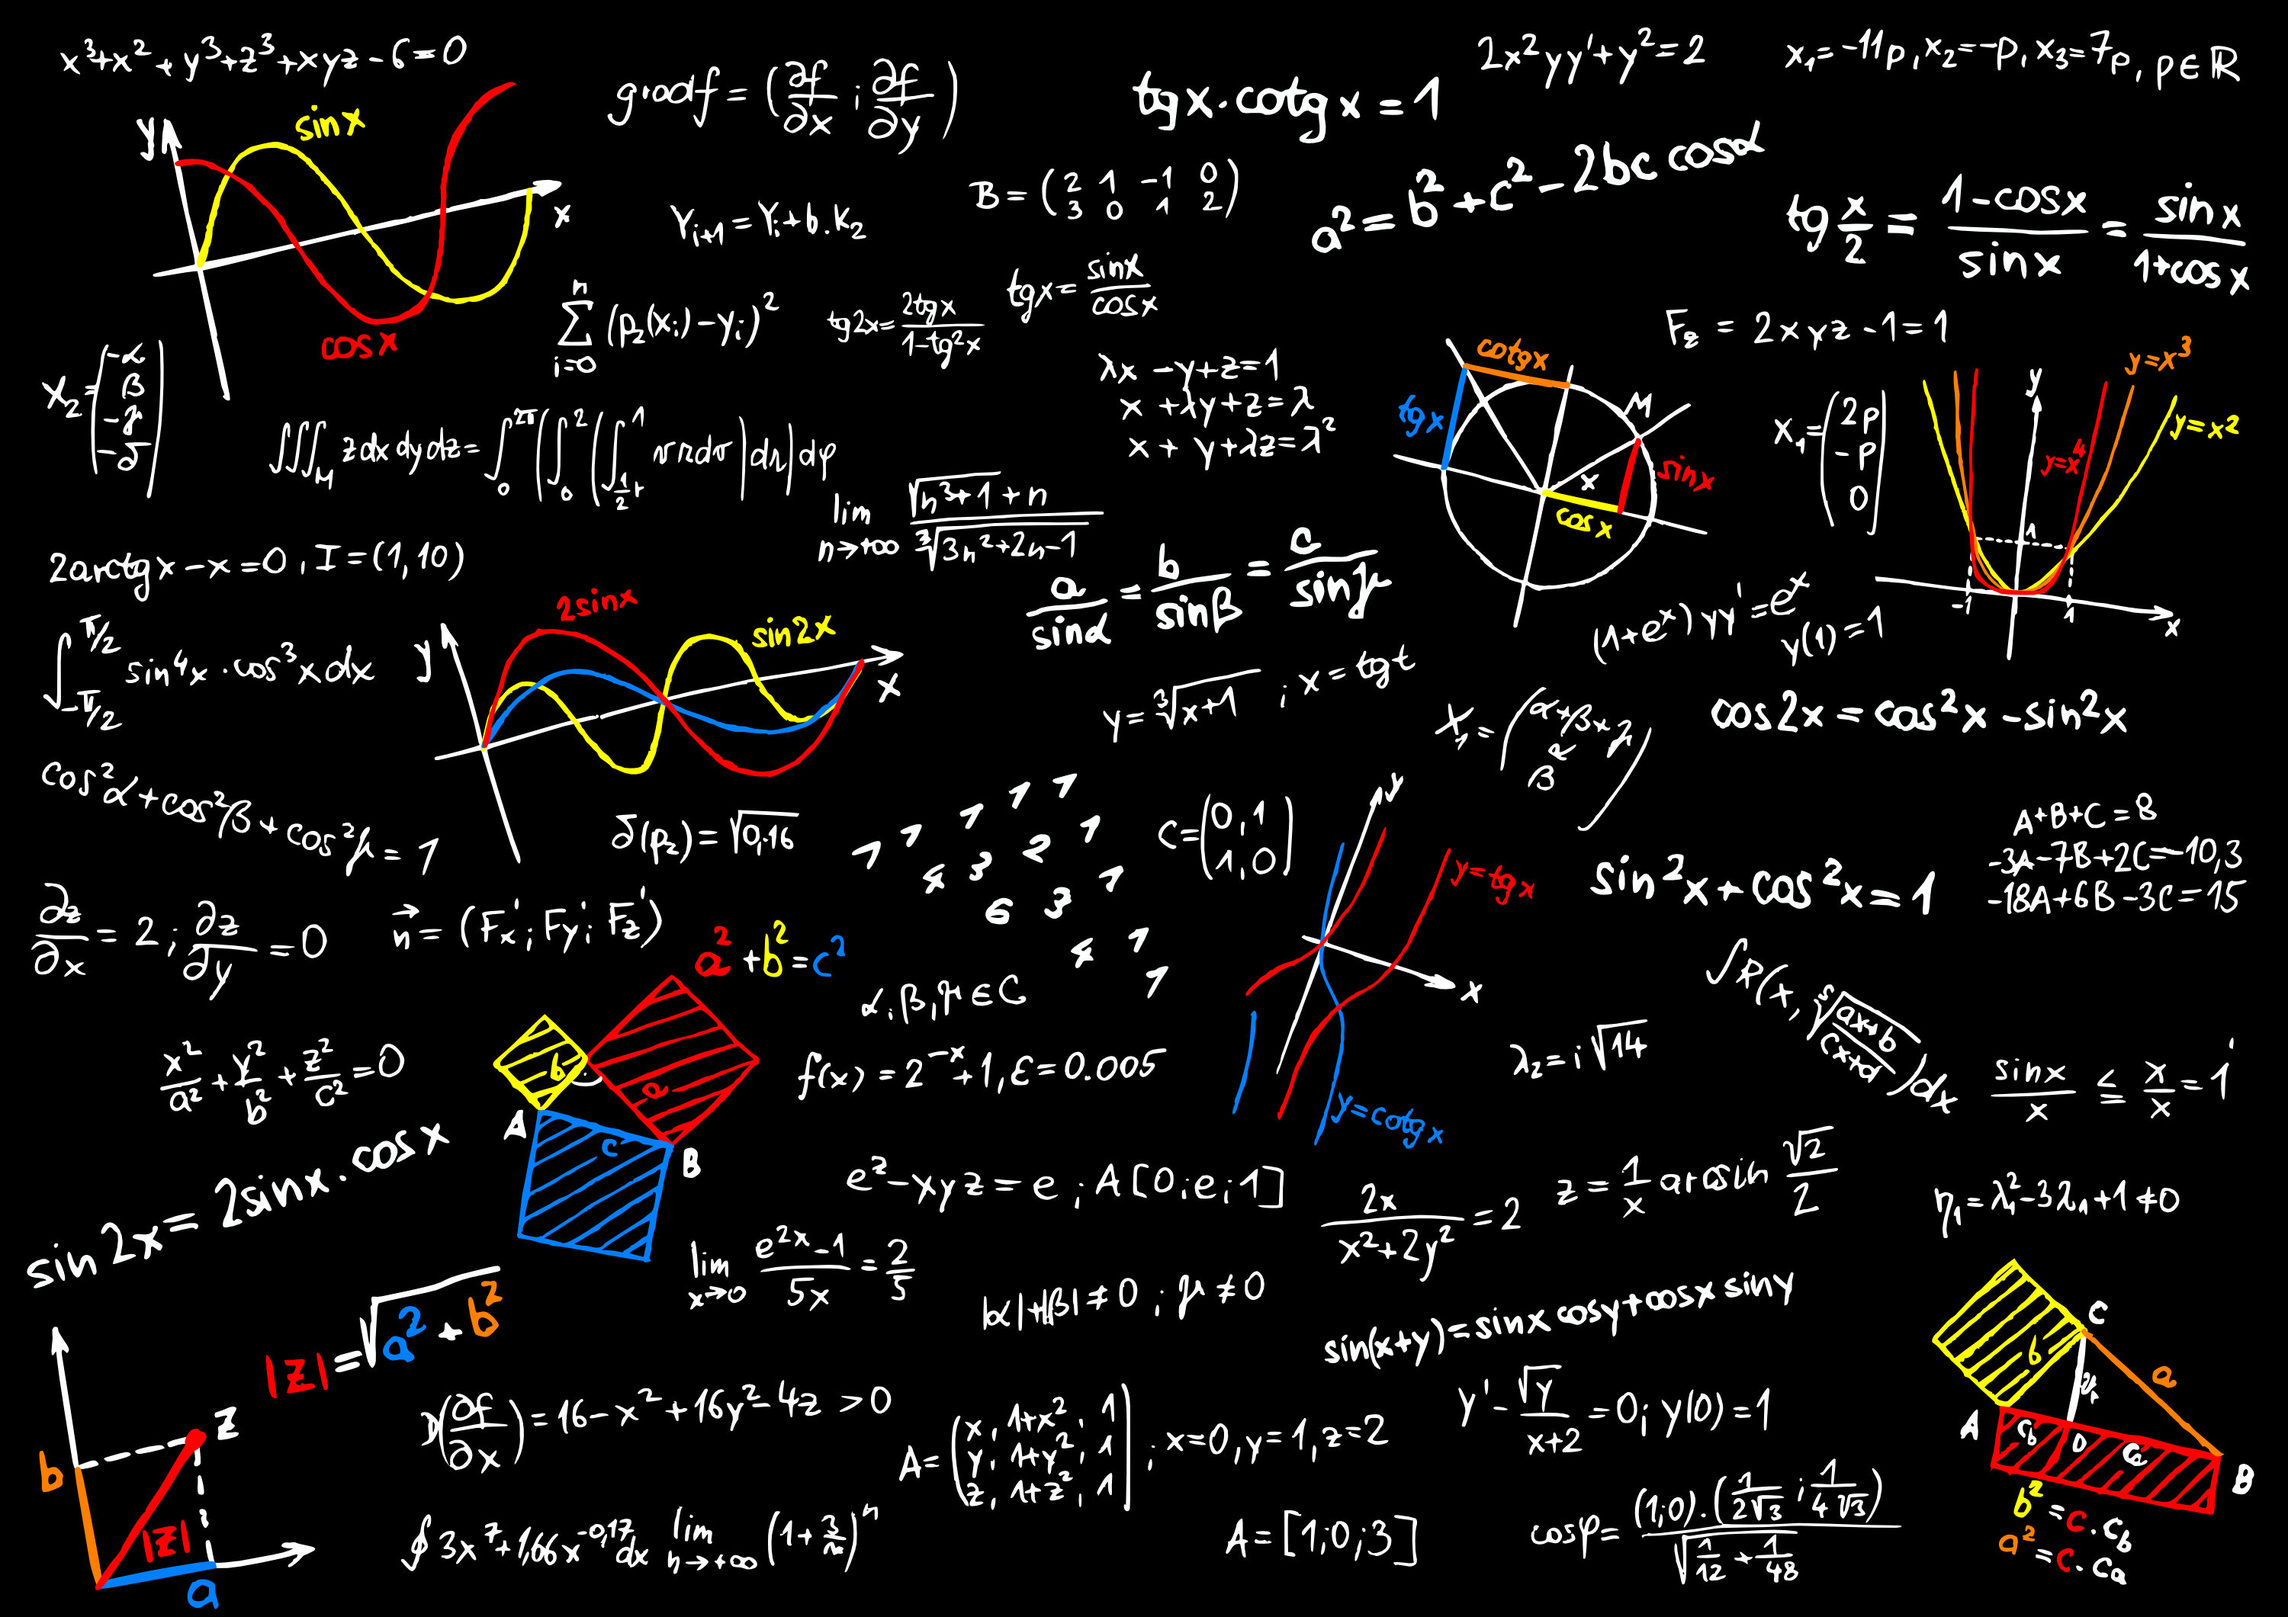
\includegraphics[width=.45\linewidth]{math}
      }
	\end{center}
\end{figure}
   
%%%%%%%%%%%%%%%%%%%%%%%%%%%%%%%%%%%%%%%%%%%%%%%%%%%%%%%%%%%%%%%%%%%%%%%%%%%%%%%
% You can insert code snippets
%%%%%%%%%%%%%%%%%%%%%%%%%%%%%%%%%%%%%%%%%%%%%%%%%%%%%%%%%%%%%%%%%%%%%%%%%%%%%%%
\newpage
\section*{Code Snippets}
\subsection*{Python}
\begin{lstlisting}
import numpy as np
import pandas as pd

def softmax(a):
    expA = np.exp(a)
    return expA / expA.sum(axis=1, keepdims=True)
\end{lstlisting}

% You can also add from a source file by uploading the file and linking it and specifying the language
% ESPECIALLY IF YOU WANT MULTIPLE LANGUAGES
\subsection*{Python from Source file}
  	% You can specify firstline and lastline as well
 	\lstinputlisting[language=Python, lastline=10]{latex_python.py} 
  
\subsection*{R}
	\lstinputlisting[language=R]{latex_R.R}
  
\end{document}